\documentclass[11pt,a4paper,titlepage,oneside]{book}

\usepackage[czech]{babel}
\usepackage[utf8]{inputenc}
\usepackage{graphicx}
\usepackage{url}
\usepackage{fancyhdr}
\usepackage{setspace}
\usepackage{hyperref}
\usepackage{rotating}


%\usepackage{titlesec}
%\titleformat{\chapter}{\normalfont\LARGE\bfseries}{\thechapter}{1em}{}
%\titlespacing*{\chapter}{0pt}{3.5ex plus 1ex minus .2ex}{2.3ex plus .2ex}


\begin{document}
%
\newcommand{\htmlTag}[1]{ \textless #1\textgreater \textless \textbackslash #1\textgreater}

%nastavení fancy stylu
\lhead{
\includegraphics[height=0.5cm]{obrazky/lev.jpg} {ČVUT v~Praze}}
\rhead{\leftmark}
\cfoot{\thepage}
\setlength{\headheight}{24pt}

\pagestyle{empty}	%%vypne číslování

\begin{titlepage} %% titulní strana 1(bez lva)
	\begin{center}
		{\huge ČESKÉ VYSOKÉ UČENÍ TECHNICKÉ} \\ [0.25cm]
		{\LARGE FAKULTA STAVEBNÍ}
		\\[9cm]		
		{\Huge DIPLOMOVÁ PRÁCE}
		\\[9cm]
		{\Large Praha 2013 \hspace{\stretch{1}} Bc. Chrudoš VORLÍČEK}
	\end{center}
\end{titlepage}

\begin{titlepage} %%titulní strana 2 (se lvem)
	\begin{center}
		{\huge ČESKÉ VYSOKÉ UČENÍ TECHNICKÉ} \\
		{\LARGE FAKULTA STAVEBNÍ \\ [0.25cm]OBOR GEOINFORMATIKA}
		\\[1cm]
		\begin{figure}[!h]
		\begin{center}
		
\includegraphics[height=5cm]{obrazky/lev.jpg}
		\\[1cm]
		\end{center}
		\end{figure}							
		{\Huge DIPLOMOVÁ PRÁCE \\ [0.25cm]}
		{\LARGE \uppercase {Prototyp turistického systému zaloŽeného na datech \\[0.25cm] OpenStreetMap}}
		\\[3.5cm]
		{\Large Vedoucí práce: Ing. Martin LANDA, Ph.D. \\[0.25cm] Katedra geomatiky}
		\\[1cm]
		{\Large Praha 2013 \hspace{\stretch{1}} Bc. Chrudoš VORLÍČEK}
	\end{center}
\end{titlepage}

\newpage %%zadání
	\begin{center}
		\vspace*{15cm}
		{\Large ZDE VLOŽIT LIST ZADÁNÍ}
	\end{center}

%% Abstrakt
\begin{flushleft}
	\chapter*{}
	\section*{ABSTRAKT}
	\paragraph{} Hlavním tématem této práce je tvorba webové turistické aplikace za použití dat OpenStreetMap, jeho napojení na sociální síť Facebook a~přidávání dat přímo do OpenStreetMap. Součástí práce je i stručné shrnutí existujích řešení, popsání užitých technologií a jejich výhod a~nevýhod.
	\section*{KLÍČOVÁ SLOVA}
	{\sc{OpenStreetMap, OSM, Turistický systém, Facebook, Nette}}
	\section*{ABSTRACT}
	\paragraph{}
	\section*{KEYWORDS}
	{\sc{}}
\end{flushleft}

\newpage %%Prohlášení
	\vspace*{15cm}
	\section*{\Large PROHLÁŠENÍ}
		\paragraph{}Prohlašuji, že jsem diplomovou práci na téma \uv{Prototyp turistického systému založeného na datech OpenStreetMap} vypracoval samostatně a~že veškerou použitou literaturu a podkladové materiály uvádím v~seznamu zdrojů.\\[1cm]
	V~Praze dne ....................... \hspace{\stretch{1}}................................. \\
	\hspace*{\stretch{1}} {(podpis autora)\hspace{0.25cm} }
	
\newpage %%Poděkování
	\vspace*{15cm}
	\section*{\Large PODĚKOVÁNÍ}
	\paragraph{}
		
\renewcommand{\baselinestretch}{1.5} %nastaví mezery
\newpage %%Obsah
\pagestyle{plain}
\pagenumbering{arabic}
\setcounter{page}{5}

	\tableofcontents

\newpage %%Obrázky a tabulky
	\listoffigures

\newpage %%Samotný text
%%Úvod
\chapter*{Úvod}
\addcontentsline{toc}{chapter}{Úvod}

%%% ML: Prvni veta zni velmi kostrbate, zvlaste "a s jeho rozšířením i
%%% do mobilních telefonů je dostupný na mnoha místech". Zkuste cely
%%% odstavec prepsat...

	\paragraph{} Internet se stal součástí životů velkého množství lidí a s jeho rozšířením i do mobilních telefonů je dostupný na mnoha místech, kde bychom ho před lety nečekaly. Díky tomu lze využívat webové aplikace ikdyž jsme na cestách. Když jsme v horách či se jen touláme přírodou, mohou nám mapové portály pomoci s plánováním další cesty. Ve srovnání s globálními navigačními satelitními systémy(GNSS) mají tyto portály jen omezené možnosti lokalizace. Webové aplikace mohou na druhou stranu poskytnout doplňující informace o zajímavých věcech, kolem kterých nás mohou naše kroky zavést. Mapové portály se pro nás staly nepostradatelným pomocníkem při plánování cest či výletů. 
	\paragraph{} Stejně tak jako se liší služební cesta od výletu, liší se i potřeby uživatelů. Podnikatel cestující autem, který hledá nejkratší cestu z bodu A do bodu B, nepotřebuje pro vyhledávání turistické mapy. Ačkoliv je může použít, obsahují pro něj nadbytečná data a mohou být příliš podrobné. Kdyby turista hledal v automapě cestu z bodu A do B, pravděpodobně by ji našel, ale vedla by nejspíš po silnicích, což není úplně žádoucí. Každá mapa, ať už papírová či internetová, poskytuje různá data. Výhodou internetových mapových aplikací je mimo jiné i možnost zobrazení různých dat v potřebném měřítku v jednom mapovém okně.

        %%% ML: Pri prvnim pouziti by mela byt zkratka rozpsana,
        %%% napr. Application Programming Interface (API). Seznam
        %%% zkratek lze generovat automaticky - viz
        %%% http://staff.science.uva.nl/~polko/HOWTO/LATEX/acronym.html

        %%% ML: Na konci odstace "Navíc se většinou jedná o
        %%% doprovodnou funkci." (ceho?) "Výhodou ovšem je snadnější
        %%% tvorba." (tvorba ceho?) Ctenar tape...

        %%% ML: Misto "prostorova data" (prilis obecny pojem)
        %%% pouzivejte radeji "geograficka
        %%% data" ci "geodata", v textu jsem to na nekolika mistech
        %%% jiz opravil

        %%% ML: Tato veta je zmatecna: "Pokud je zobrazování
        %%% geografických dat hlavní náplní aplikace, je lepší použít
        %%% specializovanou aplikaci" - v dalsim textu hovorite "o
        %%% dvou pristupech" - z textu neni zcela jasne cim se lisi
        %%% (viz poznamka vyse) Az z dalsiho textu je zrejme co mate
        %%% na mysli.

	\paragraph{} Portály poskytující mapové aplikace často vytvářejí svá API, aby jejich produkty mohly být použity i na jiných serverech. Díky tomu je možné narazit na mapy od Googlu či Seznamu i na jiných stránkách. Jedná se o nejsnažší způsob, jak prezentovat geografická data, např. společnost zabývající se venkovní reklamou tak může prezentovat rozmístění nabízených billboardů. Tento přístup má ale svá omezení daný funkcemi, které poskytuje API, a většinou i počtem přístupů či velikostí poskytovaných dat. Navíc se většinou jedná o doprovodnou funkci. Výhodou ovšem je snadnější tvorba. Pokud je zobrazování geografických dat hlavní náplní aplikace, je lepší použít specializovanou aplikaci. Vytvoření takové aplikace vyžaduje mnohem více času a znalostí. 
	\paragraph{} Pro turistiku se dají použít oba zmíněné přístupy, ovšem jejich vhodnost závisí na zamýšlených funkcionalitách. Pro zobrazení možných cílů výletů lze využít API od některého z poskytovatelů. Z českých aplikací toto využívá např. Výletník.cz \ref{sec:vyletnik}. Pokud ale chceme prezentovat síť turistických stezek, vkládat vlastní trasy, editovat data atd., je lepší vytvořit vlastní systém, ve kterém budou požadované funkce dostupné.

        %%% ML: "vytvoren" vzorek aplikaci, zkuste najit lepsi slovo

        %%% ML: "Většina nalezených aplikací neumožňuje připojení k
        %%% sociálním sítím." To je potreba nejak dolozit, mel jste na
        %%% mysli "vetsina *zkoumanych* ..."

	\paragraph{} Na internetu lze dohledat několik turistických portálů. Aby v rámci této práce nebylo vytvářeno něco, co už existuje, byl vytvořen vzorek aplikací. Tento výběr posloužil k utvoření přehledu funkcionalit, výhod, nevýhod a~originálních prvků webových mapových aplikací. Více je pospáno v kapitole \uv{Existující řešení} \ref{sec:Ex_reseni}. Většina nalezených aplikací neumožňuje připojení k sociálním sítím. V současné době, kdy jsou sociální sítě jako Facebook a~Twitter velmi rozšířené, mohou být funkce jako přihlášení přes už existující účet či sdílení výletních tras s přáteli přidanou hodnotou aplikace. 

        %%% ML: Aplikace je postavena nad daty projektu
        %%% OpenStreetMap. - to nelze definovat jako cil, a uz vubec
        %%% ne na prvnim miste, jde spise "o zakladni vlastnosti
        %%% navrzene webove aplikace, ktera vznika jako prakticky
        %%% vystup teto prace..."

	\paragraph{} Cíle této práce lze shrnout do několika hlavních bodů.
		\begin{itemize}
			\item Aplikace je postavena nad daty projektu OpenStreetMap.
			\item Pro přihlášení do aplikace lze použít účet na sociální síti Facebook. Pod tímto účtem pak lze zveřejňovat mapy na Facebooku.
			\item Přímo ze stránek projektu je možné editovat data projektu OpenStreetMap.
			\item Registrovaní uživatelé mohou přidat vlastní trasy. Jakýkoliv přihlášený uživatel může tyto trasy okomentovat.
			\item Registrovaní uživatelé mohou vkládat do mapy fotografie.
		\end{itemize}
	\paragraph{} Protože v mapách často něco hledáme, měla by vyvíjená mapa umožnit uživatelům vyhledávat objekty a cesty z bodu A do bodu B. Vyhledávání by mělo zahrnovat i pokročilé volby, kdy se dá vyhledat zájmový bod v~určité vzdálenosti od plánované cesty či od jiného bodu. Tyto body mají až druhotný význam a budou realizovány pouze v případě, že hlavní cíle projektu budou splněny.

        %%% ML: Veta "Bude zmíněna jeho historie, možnosti, kvalita a
        %%% výhody a nevýhody." zni divne, kvalita ceho...? vyhody
        %%% nevyhody - pro co? nebo silne ci slabe stranky

        %%% ML: """Množství programů a programovacích jazyků, které
        %%% lze použít, je velké." pro co? Nemel by to byt novy odstavec?

        %%% ML: piste konkretne: pouzity *pro vyvoj predkladane webobe
        %%% aplikace*, jeji vyvoj a pod

        %%% ML: Též zde lze najít popsaný výsledný stav aplikace ke dni
        %%% dokončení práce. Přeformulujte, nezni to cesky...

	\paragraph{} Práce je strukturována do pěti kapitol. V první kapitole se text věnuje existujícím řešením. Prozkoumáním aplikací bylo zjištěno, jaké funkce jsou obvykle k dispozici a jaké nikoliv. Druhá kapitola je věnována  komunitnímu projektu OpenStreetMap. Bude zmíněna jeho historie, možnosti, kvalita a~výhody a~nevýhody. Protože aplikace používá data OpenStreetMap, budou v~této kapitole popsána. Třetí kapitola je zaměřena na technologickou stránku problému. Množství programů a programovacích jazyků, které lze použít, je velké. Proto v této části budou popsány jen ty programy, jazyky a~knihovny, které se použily či  jejichž použití bylo zvažováno. Ve čtvrté části práce je popsán vývoj a s ním spojené problémy. Též zde lze najít popsaný výsledný stav aplikace ke dni dokončení práce. V poslední, páté kapitole je zhodnocení celého projektu, odůvodnění koncového stavu a nápady na rozšíření, vylepšení či dodělání aplikace.
	
\pagestyle{fancy}

%%%%%%%%%%%%%%%%%%%%%%%
%%%%% EXISTUJÍCÍ ŘEŠENÍ 	   %%%%%
%%%%						      %%%%
%%%							  %%%
%%								     %%
%									 %
\chapter{Existující řešení}
	\label{sec:Ex_reseni}
	\paragraph{} Z velkého množství různých mapových aplikací bylo vybráno šest zástupců, kteří mají alespoň nějakou spojitost se zpracovávaným tématem. Kromě dvou v České republice nejčastěji užívaných mapových portálů GoogleMaps a Mapy.cz byly pro hodnocení zvoleny tři aplikace postavené nad daty OpenStreetMap. Jedná se o české aplikace OpenTrackMap a MTB mapa Evropy. Trojici uzavírá web Waymarked Trails. Poslední aplikací je už v úvodu zmiňovaný Výletník.cz, jehož mapová aplikace je vytvořena pomocí Google API. Každá z těchto aplikací je něčím specifická, má své výhody i nedostatky. 
	\section{Google Mapy}
		\url{http://www.google.com/maps/preview}

                %%% ML: nektere pojmy by bylo zahodno vysvetlit, napr. Street View
                
                %%% ML: jaka data lze napriklad sdilet

		\paragraph{} V globálním měřítku asi nejužívanější mapovou aplikací jsou Google Mapy spuštěné v roce 2005. Ve stejném roce společnost Google uvedla k mapám i API pro jejich použití na webech třetích stran. Podle typu užití se jedná buď o placenou či volně dostupnou službu. Google má k mapám velké množství doplňkových funkcí -- od vyhledávání míst přes vyhledávání cest autem, na kole či pěšky po Street View, zobrazení 3D modelů budov a fotografií z~momentálně zobrazené oblasti. Též lze importovata svá data a sdílet je s~jinými uživateli.

                %%% ML: "která je na s mapami provázána" ??? 

		\paragraph{} Google Mapy sice jsou užitečným pomocníkem při plánování cest a zobrazení prostorových dat, ovšem jejich užití je pro turisty dosti omezené. Aplikace nedisponuje údaji o turistických stezkách. Důvodem, proč se mapy od Googlu dostaly do tohoto výběru, je aplikace Panoramio, která je na s mapami provázána. Jedná se vrstvu lokalizovaných fotografií, které uživatelé nahrály do aplikace. Možnost nahrát fotky do mapy sice poskytují i  Mapy.cz, ovšem aplikace Panoramio je starší -- vznikla v roce 2005. Původně nebyla vlastněna Googlem, ten ji získal v roce 2007 a v roce 2008 byla propojena s~mapovou aplikací. 

                %%% ML: chybi vystleni zkraek, WGS, EPSG a pod

		\paragraph{}  Google vytvořil pro své mapy i nové zobrazení, které vychází z Mercatorova zobrazení. Pro zobrazení jsou použity vzorce pro Mercatorovo zobrazení na kouli, ale objekty mají  souřadnice v systému WGS 84, což vede k tomu, zobrazení není konformní.\label{google_mercator} Toto zobrazení má v označení EPSG:900913.

		\begin{figure}[!h]
			\begin{center}
				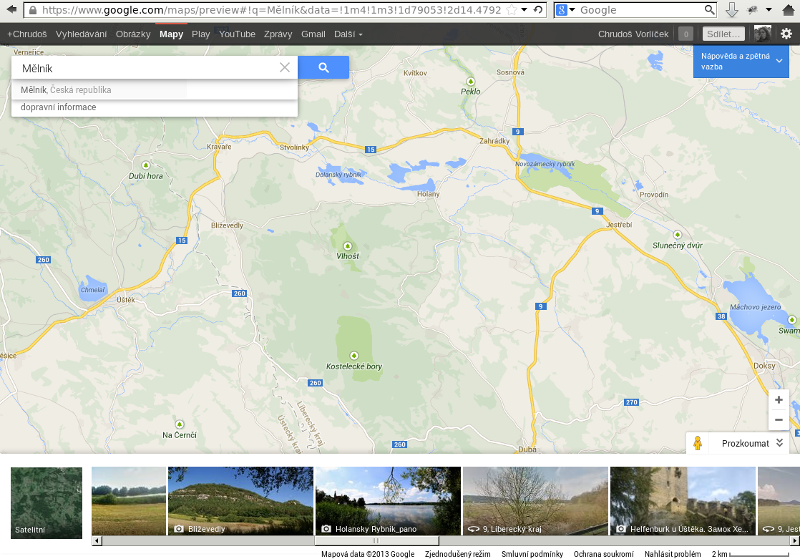
\includegraphics[width=12cm]{obrazky/googleMaps.png}
				\caption{Google Mapy s přehledem obrázků}
			\end{center}
		\end{figure}

			\begin{figure}[!h]
				\begin{center}
					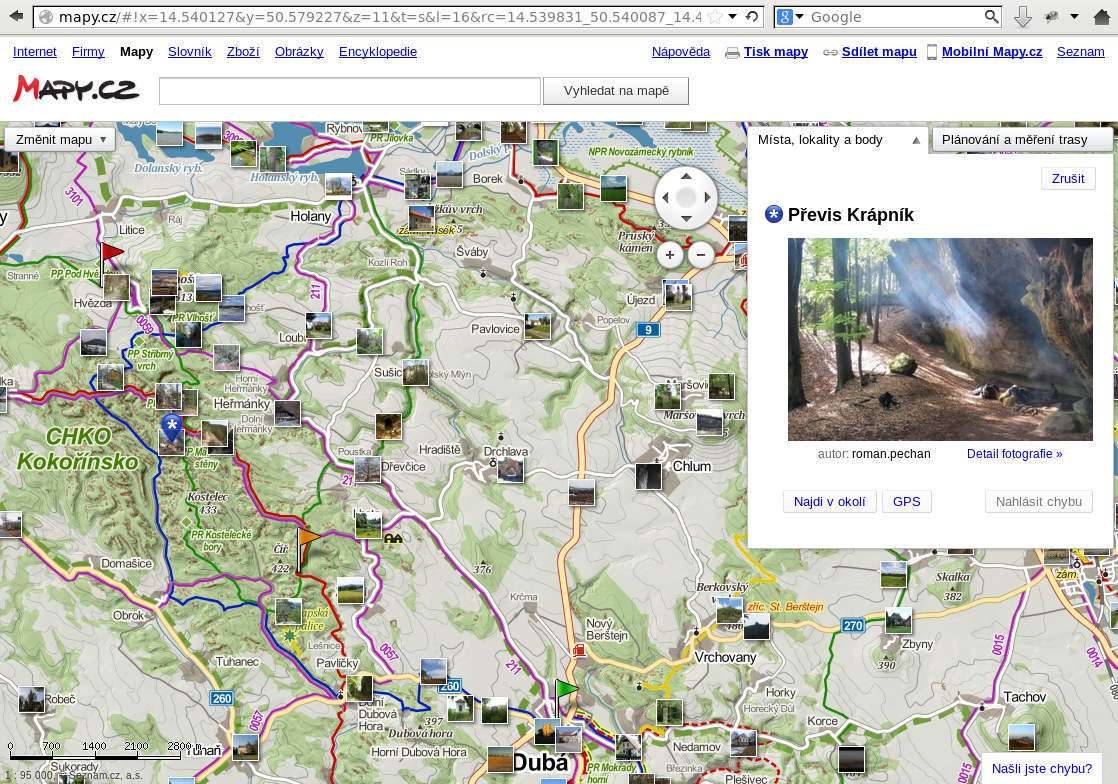
\includegraphics[width=12cm]{obrazky/mapycz.png}
					\caption{Turistická mapa na Mapy.cz}
				\end{center}
			\end{figure}

	\section{Mapy.cz}
		\url{http://mapy.cz/}
		\paragraph{} I když je Google se svými mapami světově nejužívanější, v českých pod\-mínkách mu směle konkuruje mapová aplikace firmy Seznam. Mapy.cz mají oproti Googlu výhodu domácího prostředí a zaměření zejména na Českou republiku, což v důsledku znamená rychlejší aktualizaci mapových podkladů. Mapy.cz poskytují tři různé podkladové mapy (leteckou, obecnou a turistickou) a různé tématické vrstvy (turistické trasy, cyklotrasy, dopravní info, zastávky MHD a veřejné dopravy aj.). 
		\paragraph{} Na Mapách.cz mohou řidiči, cyklisti a chodci vyhledat trasy z bodu A do bodu B přes libovolný počet mezilehlých bodů. V závislosti na zvoleném dopravním prostředku bere vyhledávač v potaz i lesní cesty a turistické trasy. Ve stejné záložce lze najít i ruční měření vzdálenosti. Vyhledaná či ručně zadané cesta může být exportována. Též lze zobrazit její výškový profil. Do mapy lze přidat vlastní body a ty sdílet s ostatními uživateli pomocí URL adresy. Stejně jako Google poskytuje i Seznam možnost vyhledávat místa podle souřadnic, ulice či názvu objektu. Mapy.cz podporují vkládání fotografií a jejich komentování, ale narozdíl od Googlu to není řešené jinou aplikací, ale je to přímo součástí aplikace.

		\begin{figure}[!h]
			\begin{center}
				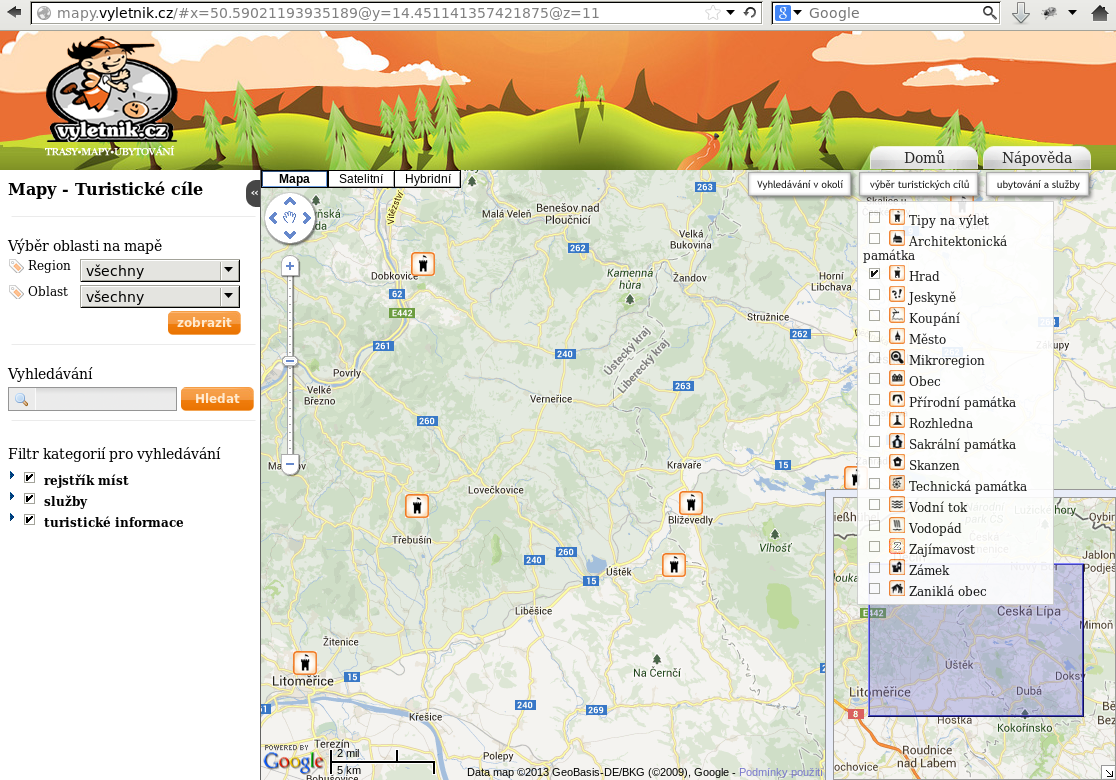
\includegraphics[width=12cm]{obrazky/vyletnik.png}
				\caption{Mapová aplikace portálu Výletník}
			\end{center}
		\end{figure}

	\section{Výletník}
		\label{sec:vyletnik}
		\url{http://mapy.vyletnik.cz/}
		\paragraph{} Turistický portál Výletník.cz poskytuje informace o možných cílech výletů, o službách spojených s turistikou (např. restaurace či ubytování)  či o zají\-mavých akcích. Díky těmto datům je portál dobrým zdrojem nápadů, pokud připravujeme výlet. Registrovaným uživatelům poskytuje portál informace o akcích probíhajících následující víkend. Též uživatelům umožňuje vkládat vlastní fotografie, místa a příspěvky. Při registraci je inzerována možnost registrace pomocí Facebooku, ale nikde na to nebyl nalezen odkaz. Nakonec se ukázalo, že Adblock, doplněk prohlížeče Firefox blokující reklamy, vyhodnotil přihlašovací nástroj pro Facebook jako reklamu a podle toho s ním zacházel. Po vypnutí Adblocku propojení s Facebookem bylo viditelné. Na druhou stranu se objevilo množství reklam, které kazí jinak dobrý pocit z webu.
		\paragraph{} Pro mapovou aplikaci tohoto portálu platí to, co pro celý web -- všudy\-přítomné reklamy snižují přívětivost aplikace. Na několika místech se projevilo špatné nastylování aplikace, kdy se prvky překrývaly. Nejzřetelněji je to vidět na možnosti přepínání map. V nápovědě je napsáno, že aplikace poskytuje normální, satelitní a hybridní podkladovou mapu, ale možnost přepínání těchto map je překryta rozbalovacími seznamy zájmových bodů. Těch je k dispozici velké množství a jsou rozděleny na dvě základní skupiny -- \textit{turistické cíle} a \textit{ubytování a služby}. Obě skupiny obsahují další možnosti, ze kterých lze zvolit jednu či více položek. Výletník.cz umožňuje uživatelům vyhledávat objekty ve třech kategoriích:
			\begin{itemize}
				\item rejstřík míst,
				\item služby,
				\item turistické informace.
			\end{itemize}
Vyhledávat lze i v určitém okruhu od zvoleného bodu.
		\paragraph{} Ačkoliv tato aplikace poskytuje solidní informace, má jistá omezení vyplí\-vající z toho, že je vytvořena pomocí GoogleMaps API. Jednou z nevýhod jsou chybějící turistické a cykloturistické trasy. Google mapy tyto informace neposkytují a aplikace samotná je z jiných zdrojů nezískává, čímž vzniká nutnost pro užití dalších portálů pro plánování výletu.	
	
	\section{Waymarked Trails}
		\url{http://waymarkedtrails.org/cs/}

                %%% ML: "Největší množství dat je v Evropě, zbylé
                %%% části světa jsou z velké části bez dat, ikdyž
                %%% občas nějaká data obsahují. Nejvíce dat je
                %%% poskytují vrstvy s turistickými a
                %%% cykloturistickými stezkami" - zkuste cele
                %%% preformulovat, nezni to prilis cesky

		\paragraph{} Aktuální přehled stezek pro turistiku, cykloturistiku a jízdy na inline bruslích je možno najít na mapě Waymarked Trails\cite{Waymarked}. Tato aplikace je vytvořena nad daty \textit{OpenStreetMap} a pokrývá celý svět. Největší množství dat je v Evropě, zbylé části světa jsou z velké části bez dat, ikdyž občas nějaká data obsahují. Nejvíce dat je poskytují vrstvy s turistickými a cykloturistickými stezkami. O poznání menší množství dat poskytují vrstvy pro horskou cyklistiku a inline bruslení.

		\begin{figure}[!h]
			\begin{center}
				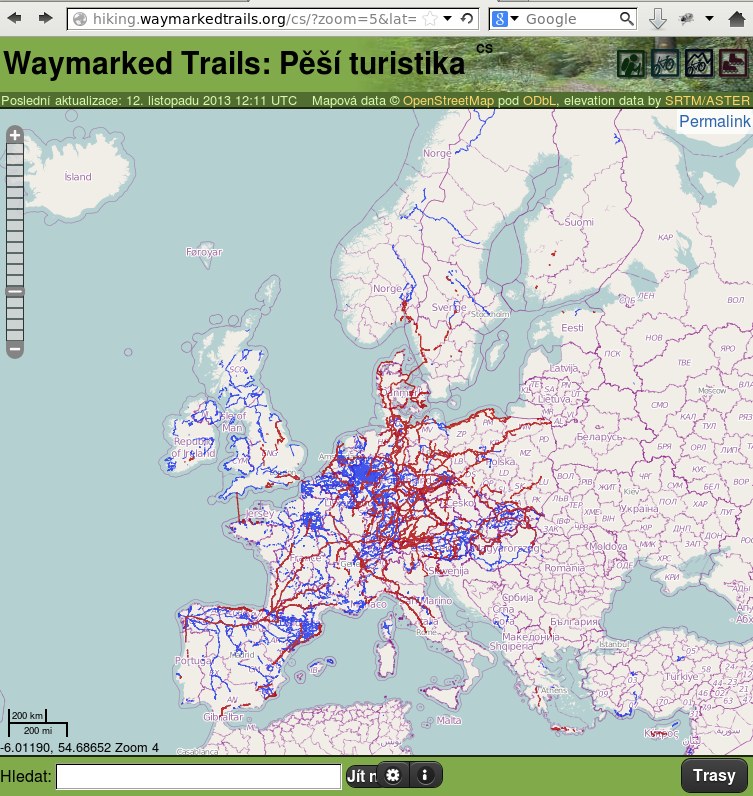
\includegraphics[width=8cm]{obrazky/waymarkedTrails.png}
				\caption{Hiking Map na Waymarked Trails}
			\end{center}
		\end{figure}
	
		\paragraph{} Velkou výhodou této mapy je poskytování informací o trasách a možnost jejich uložení v GPX formátu. Trasy jsou rozděleny na:
	\begin{itemize}
		 \item kontinentální -- mezinárodní trasy vedoucí přes několik států, značené prefixem E
		 \item národní -- trasy KČT
		 \item regionální -- trasy KČT
     		 \item ostatní -- naučné stezky, odbočky k hradům, zříceninám, vyhlídkám, přírodním zajímavostem apod.
	\end{itemize}
  Mapa také poskytuje možnost vyhledání místa podle názvu a vytvoření permanentního odkazu na mapový výřez. Mapa neposkytuje vyhledávání tras -- na to je potřeba použít jiná existující řešení, např. OpenRouteService (\url{http://www.openrouteservice.org/}), které kromě vyhledání trasy pro určitý typ dopravy (autem, na kole, pěšky) poskytuje i její export, výškový profil, vyhledání zájmových bodů v blízkosti.

 	\section{OpenTrackMap}
		\url{http://opentrackmap.cz/}

                %%% ML: nerekl bych "ze odpada problem s licenci",
                %%% spise ze "licence ODBL umoznuje pouziti dat OSM
                %%% pro tyto typy aplikaci"
                
                %%% ML: chybi odkaz na Mapnik, slovo "zobrazeni" je v
                %%% teto souvislosti zavadejici

		\paragraph{} OpenTrackMap je projekt Ing. Radka Bartoně. Projekt běží na serveru geo102, který spravuje katedra Geomatiky na Fakultě stavební ČVUT v~Praze. Tvorba této aplikace byla motivována snahou poskytnout mapy pro aplikaci TangoGPS běžící na platformě Openmoko\cite{OTM}. Již existující mapy nemohly být z licenčních důvodů či kvůli různým technickým omezením použity. Data OpenStreetMap mohou být volně použity, tudíž zde odpadá problém s licencí. Data jsou uložena v databázi PostgreSQL a pro jejich zobrazení je použit software Mapnik. Ačkoliv mapy v současné době nejsou aktualizovány, jejich přínos je ve vytvoření značkového klíče pro tras a objektů v~mapě. 

		\begin{figure}[!h]
			\begin{center}
				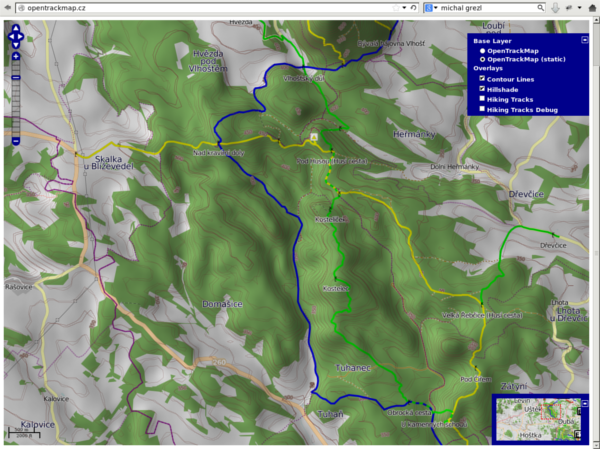
\includegraphics[width=12cm]{obrazky/otm.png}
				\caption{OpenTrackMap}
			\end{center}
		\end{figure}

                %%% ML: chybi citace, odkud jste toto cerpal, v textu
                %%% vubec chybi odkazy na literaturu, clanky ze
                %%% kterych jste cerpal!!! zkuste jich par doplnit, to
                %%% je celkem ZASADNI nedostatek...

		\paragraph{}  Aplikace poskytuje vrstevnice, stínování terénu, podkladovou mapu a turistické trasy. Vzhledem k tomu, že mapy byly určeny pro zobrazení v mobilních zařízeních, bylo zapotřebí snížit množství dat přenášených k uživateli. Toho bylo dosaženo pomocí dlaždic. Původní testování odhalilo, že pro malá měřítka je vykreslování pomalejší, protože je pro velkou oblast vykreslováno stínování kopců. Od určitého stupně přiblížení se rychlost vykreslení mírně zvýšila, protože byla vykreslována menší plocha a protože klesl počet vektorových prvků.

	\section{MTB mapa Evropy}
		\url{http://mtbmap.cz/}
		\paragraph{} Projekt Martina Tesaře MTB mapa Evropy byl původně bakalářskou prací zpracovávanou na fakultě informatiky Masarykovy univerzity v Brně. Aplikace prezentuje stezky pro jízdu na horském kole. Mapa byla původně omezena pouze na oblast České republiky a přilehlého okolí, ale časem byla rozšířena na Evropy. Mapa využívá značkový klíč projektu OpenTrackMap, který je popsán na OpenStreetMap Wiki\cite{otm_klic}, a kromě cyklistických stezek zobrazuje i turistické cesty. Aktuálnost mapy je udržována týdenními aktualizacemi dat OpenStreetMap. Data pochází ze serveru \textit{geofabrik.de}, který poskytuje možnost stažení dat OpenStreetMap pro jednotlivé země, kontinenty i celý svět.

                %%% ML: prvni veta zni divne...

                %%% ML: co umoznuje sluzva Nominatim vyhledavat? v
                %%% dalsim textu to mate zmineno, ctenar musi ale
                %%% patrat

                %%% ML: co je editor iD, vysvetlit...

		\paragraph{} Aplikace poskytuje velké množství funkcí, které jsou dostupné všem. K dispozici je vyhledávání pomocí služby OpenStreetMap Nominatim\cite{nominatim}. Dále lze exportovat data v souřadnicemi daném výřezu. Zde lze nastavit stupeň přiblížení, velikost výsledku v pixelech a zobrazené mapové prvky -- tiráž, název mapy, trasu, legendu a měřítko. Kromě vyhledávání míst  pomocí Nominatim je k dispozici i vyhledání cesty podle množství vstupních parametrů, které zahrnují například typ cesty, druh povrchu nebo obtížnost. Tyto parametry jde uložit na disk a později je znovu použít pro vyhledání stejné cesty. Lze též vložit vlastní cestu v souboru GPX nebo ručně a zobrazit k ní výškový profil. Takto vytvořené stezky se zobrazí v mapě, ale neukládají se pro pozdější zobrazení. Aplikace umožňuje vygenerovat permanentní odkaz na zobrazenou pozici či přesměruje uživatele na OpenStreetMap a otevře editor iD.

                %%% ML: co je EPSG:3857 nejde jenom o kartograficke
                %%% zobrazeni, mluvil bych spise o souradnicovem
                %%% systemu

		\paragraph{} Tento projekt má svoji stránku i na OpenStreetMap Wiki, kde jsou popsány úkoly, kterými by měl směřovat další vývoj aplikace. Mapa byla původně vytvořena v OpenLayers\cite{tesar_bp}, ale v současné době užívá javascriptovou knihovnu Leaflet. K dispozici jsou 4 podkladové mapy (MTB mapa, OSM Mapnik, OpenCycleMap, Hike \& Bike Map), které jsou zobrazeny v EPSG:3857. Toto zobrazení je ekvivalentní s EPSG:900913, které na svých mapách používá Google. Jak bylo uvedeno výše \ref{google_mercator}, toto zobrazení není přesně konformní, ovšem v tiráži je uvedeno \uv{Zobrazení: Konformní válcové - mercatorovo}.
		\begin{figure}[!h]
			\begin{center}
				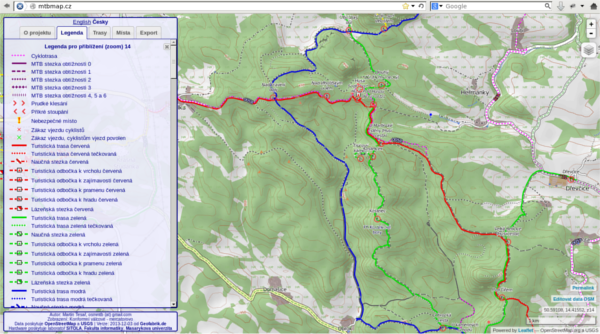
\includegraphics[width=12cm]{obrazky/mtb.png}
				\caption{MTB mapa Evropy}
			\end{center}
		\end{figure}

%%%%%%%%%%%%%%%%%%%%%%%
%%%%% OPEN STREET MAP        %%%%%
%%%%						      %%%%
%%%							  %%%
%%								     %%
%									 %
\chapter{OpenStreetMap}
	\section{O Projektu}

        %%% ML: "a toto jméno se zde velice často objevuje" zni
        %%% opravdu spatne..., zduvodneni formulovane jako "Z toho
        %%% důvodu by bylo vhodné říci o co se jedná" je potreba
        %%% preformulovat, neco jako "cilem kapitoly je ...."

		\paragraph{} Tato práce je navázána na projekt OpenStreetMap a toto jméno se zde velice často objevuje. Z toho důvodu by bylo vhodné říci o co se jedná, jakou má projekt historii, jak v současné době vypadá a jaké má využití. 

                %%% ML: "OpenStreetMap je svobodná mapa" je
                %%% zavadejici, nepresne a divne..., zkuste tuto cast
                %%% prepsat, opet chybejeji citace jako v celem textu...

                %%% ML: nejde o "mapove dilo" !!! jaka jina "mapova
                %%% dila" mate na mysli

                %%% ML: "stahnout si data" jaka data - neni vysvetleno

                %%% ML: OSM jiz nepouzivat CC-BY-SA !!! -
                %%% http://wiki.openstreetmap.org/wiki/Cs:ODbL/We_Are_Changing_The_License
                %%% opet chyby jakakoliv reference ... (!!!)

		\paragraph{} OpenStreetMap je svobodná mapa, kterou vytváří a spravují její uživatelé. Narozdíl od jiných mapových děl OpenStreetMap poskytují uživatelům možnost stáhnout si data a volně s nimi nakládat. Díky možnosti svobodného nakládání s daty vznikají různá mapová díla dle potřeb uživatelů. Mapa musí mít uvedeno autorství OpenStreetMap contributors a musí být šířena pod stejnou licencí jako samotná OpenStreetMap. Toto je známo jako licence \textit{CC BY-SA 2.0}\cite{creative_commons}.
		\paragraph{}Projekt vznikl ve Velké Británii v roce 2004. O jeho základy se postaral Steve Coast, který se nechal inspirovat jiným komunitou řízeným projektem -- svobodnou encyklopedií Wikipedie. O dva roky později vznikla OpenStreetMap Foundation, která projekt podporuje. V průběhu let povolily některé společnosti používat své mapové podklady pro tvorbu OpenStreetMap. V roce 2006 to byl Yahoo. O rok později Automotive Navigation Data poskytla mapy silniční sítě Nizozemska, Indie a Činy. 
		\paragraph{} Od vzniku aplikace vzrostl počet registrovaných uživatelů až na milion. V~srpnu 2008 měla aplikace 50 000 registrovaných uživatelů. Do konce násle\-dujícího roku narostlo toto číslo na skoro na  200 000. V roce 2012 služba registrovala 600 000 členů a 6. ledna 2013 překročil počet uživatelů 1 milion. Ze statistik vyplývá, že kolem 30\% uživatelů vytvořilo alespoň jednu sadu změn\cite{neis}.

                %%% ML: kazdy obrazek musi byt uveden zdroj !!!
                
                %%% ML: obrazek ma nevhodny popisek - uzivatelu ceho?
                %%% (je potreba uvest OSM), v seznamu obrazku to bude matouci

		\begin{figure}[!h]
			\begin{center}
				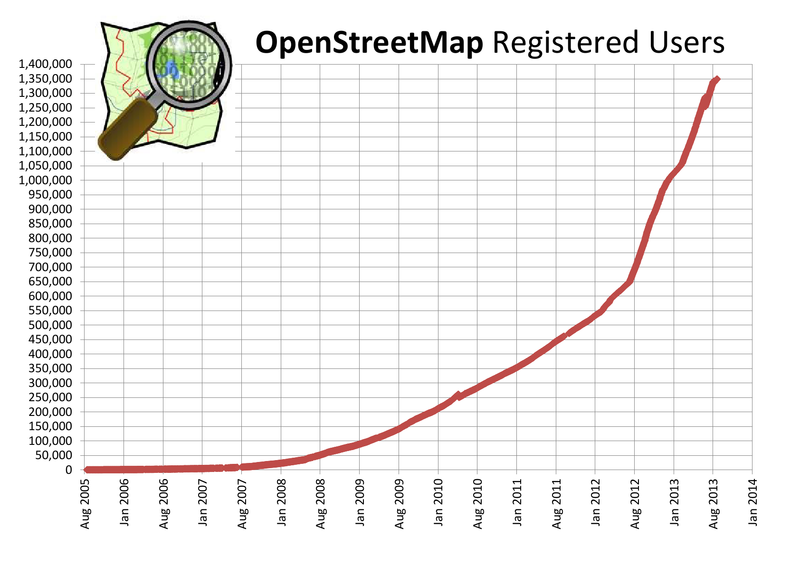
\includegraphics[width=12cm]{obrazky/osm_stat_users.png}
				\caption{Graf nárustu registrovaných uživatelů}
			\end{center}
		\end{figure}

                %%% ML: jaka data? prilis obecne

	\section{Data}
		\subsection{Typy dat}

                %%% ML: rozlicnych dat ci kvalitu dat, ci neco jineho
                %%% ??? nepresna formulace

                %%% ML: "standardnich objektu" to je velmi nepresne,
                %%% silnice ci vodstvo nejsou objekty...

                %%% ML: co mate na mysli "normalnimi mapami" ? je
                %%% treba to nejak rozvest...

                %%% ML: "Data mohou byt" zni divne, spise neco jako
                %%% "Rozlisuje tri zakladni elementy datoveho modelu,
                %%% ktery projekt OSM pouziva:" ci neco podobnebo

		\paragraph{} Jak už bylo řečeno, data pořizují samotní uživatelé mapy, což má za následek velké množství rozličných dat. Kromě standardních objektů, jako jsou silnice, vodstvo, budovy, zalesněné oblasti či turistické značky, jsou mapovány i věci, které na normálních mapách zobrazeny nejsou. Jedná se například o bezpečnostní kamery na veřejných místech. Data mohou být:
	\begin{itemize}
		\item uzly (nodes) -- body se souřadnicemi,

                  %%% ML: nebo co?

		\item cesty (ways) -- liniové prvky a hranice polygonů -- nebo

                  %%% ML: jakymi dalsimi prvky?

		\item relace (relations) -- popisují vztahy s dalšími prvky.
	\end{itemize}
Kromě těchto tří elementů mohou mít prvky své tagy, do kterých se zaznamenávají  vlastnosti. 	

%%% ML: "nebo jsou součástí cesty" zni divne, mate na mysli, ze uzly
%%% tvori lomove body cesty? nebo jenom pocatecni a koncovy bod cesty
%%% (lomene cary) ?

		\paragraph{}Uzly mají přiřazeny zeměpisné souřadnice a identifikátor (id). Volitelně může být prvku přiřazena i výška. Uzly mohou být samostatné prvky (např. rozcestník či sloup) nebo jsou součástí cesty. V tom případě definují tvar cesty. Uzly musí být na spojnicích více cest -- např. když se protínají dvě cesty, tak součástí obou cest musí být stejný vrchol. Pokud by to tak nebylo, nejednalo by se z topologického hlediska o křižovatku, ale mimoúrovňové křížení. Globální dataset obsahuje k roku 2013 přes 2 x 10$^9$ uzlů.

%%% ML: chybi zdroj, to musite uvest...

		\begin{figure}[!h]
			\begin{center}
				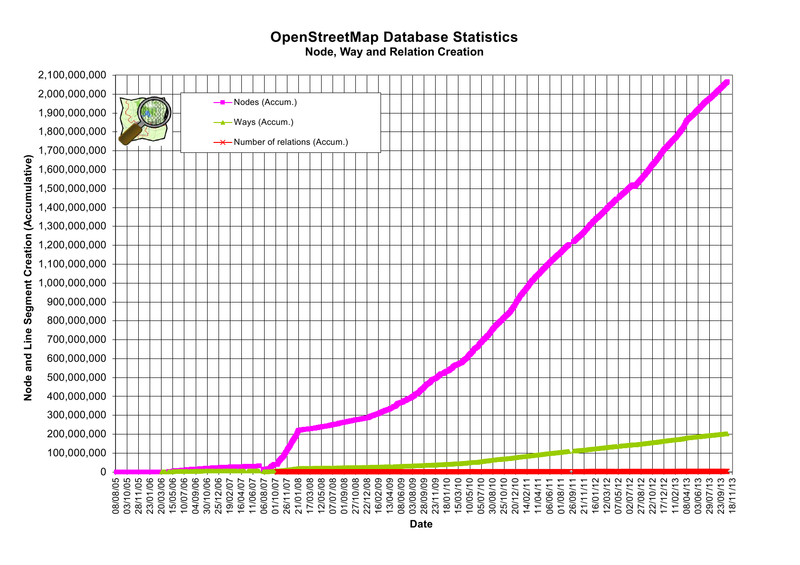
\includegraphics[width=12cm]{obrazky/osm_stat_elements.png}
				\caption{Graf vývoje počtu uzlů, cest a relací}
			\end{center}
		\end{figure}

                %%% ML: "Oproti uzlům je cest výrazně míň" to nezni
                %%% prilis staste, zkuste preformulovat, jedna se o
                %%% text technickeho charakteru

		\paragraph{} Oproti uzlům je cest výrazně míň (kolem 200 000), protože cesty jsou tvořeny 2 až 2000 uzly spojenými liniovými segmenty. Cesta je buď otevřená nebo uzavřená. Otevřená cesta je taková, kde začátek a konec tvoří jiný uzel. Uzavřená cesta má identický počáteční a koncový uzel. V tomto případě se může jednat o uzavřenou polylinii či plošný prvek. Rozdíl lze stanovit pomocí tagu area -- pokud má hodnotu yes, jedná se o plochu. V některých případech může cesta tvořit polylinii a hranici polygonu zároveň -- toto je pak označeno odpovídajícím způsobem ve vlastnostech.

		\begin{figure}[!h]
			\begin{center}
				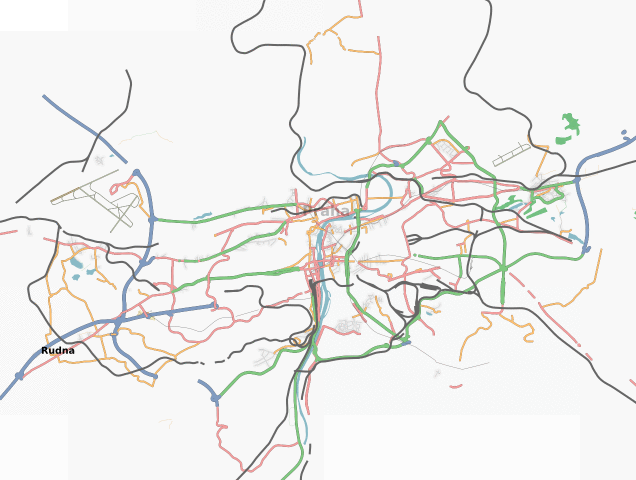
\includegraphics[width=12cm]{obrazky/Osm-200607-praha.png}
				\caption{Praha na mapách OpenStreetMap -- červenec 2006}
				\label{fig:praha2006}
			\end{center}
		\end{figure}

                %%% ML: "Vznik dat" divne, zkuste preformulovat - zdroje dat

                %%% ML: "chodi venku" nezni jako formulace s diplomove prace

                %%% ML: "souradnice, ktere pak importuje v souboru GPX
                %%% do mapy" zni opet divne, tuto formulace by me
                %%% neprekvapila jinde, ale u zaverecne prace oboru
                %%% "geoinfomatika" ano, zkuste prepsat

                %%% ML: Druhou "variantou" jako variantou, dalsim zdrojem dat ....

		\paragraph{} Vznik dat se dá rozdělit do tří skupin. První z nich je přímý sběr v terénu, kdy uživatel chodí venku a pomocí GPS přístroje získává souřadnice, které pak importuje v souboru GPX do mapy. Druhou variantou je odvozování z existujících mapových děl. Zde je ovšem potřeba dávat pozor, aby podklady pro odvození  byly kompatibilní s licencí, kterou užívá OpenStreetMap. V~případě, že nejsou vyjasněny licenční podmínky, materiály použity být nemohou. Pro odvozování na území České republiky se dá kupříkladu použít ortofoto poskytované přes WMS Ústavem pro hospodářskou úpravu lesů (ÚHÚL) či WMS katastrální mapy Českého úřadu zeměměřického a katastrálního (ČÚZK). WMS ortofotomapy ČÚZK na odvozování nemůže být použita. Může být ale použita na ověření přesnosti jiných použitelných zdrojů.

                %%% ML: opet chybi zdroj

		\begin{figure}[!h]
			\begin{center}
				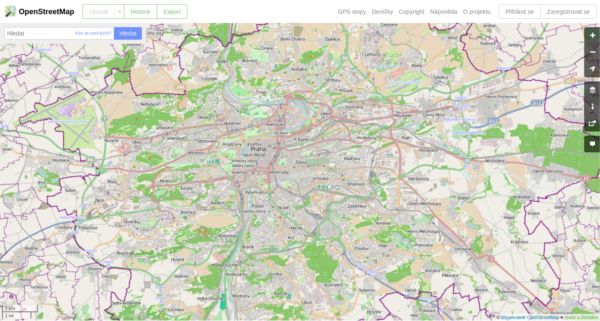
\includegraphics[width=12cm]{obrazky/Osm-201312-praha.png}
				\caption{Praha na mapách OpenStreetMap -- prosinec 2013}
				\label{fig:praha2013}
			\end{center}
		\end{figure}


                %%% ML: chybi odkaz na graf, ctenar musi hledat...

                %%% ML: konec odstavce: "zatímco druhý obrázek je
                %%% plnohodnotnou mapou." je spatna formulace, obrazek
                %%% muze byt tezkou mapou, 

		\paragraph{} Graf vývoje počtu elementů ukazuje, že z počátku přibývalo malé množství objektů a větší zvrat nastal spolu s nárustem počtu uživatelů. V roce 2007 je vidět skokový nárust počtu bodových prvků -- jedná se o data silniční sítě Nizozemska, Indie a Číny poskytnuté organizací Automotive Navigation Data. 
		Přibývání počtu prvků v mapě lze též dobře sledovat na malých plochách. Pro ilustraci jsou zde přiloženy obrázky, jak Praha byla zmapována v roce 2006 \ref{fig:praha2006} a v prosinci 2013 \ref{fig:praha2013}. V prvním případě jsou zmapovány hlavní silnice a vodní toky, zatímco druhý obrázek je plnohodnotnou mapou.
	
	\subsection{Uložení dat}
		\paragraph{} Data se ukládají do databáze, která je klíčovým prvkem celého projektu. Pro každý typ prvku existují tabulky v databázi. Kromě současné verze obsahuje databáze i historické verze, takže lze dohledat změny a případně je vrátit. Další tabulky se vztahují ke změnovým sadám (changesetům), GPX souborům nebo registrovaným uživatelům. Kromě tabulek jsou uloženy i primární a cizí klíče, sekvence a indexy.

                %%% ML: "extrakt" neni rozhodne ceske slovo... zkuste
                %%% najit lepsi termin, dale pouzivate "vytahy" coz
                %%% neni take uplne stastny termin

		\paragraph{} Data jsou distribuovány v XML souboru Planet.osm, který je vytvářen v~týdenních intervalech. V současnosti je velikost nekomprimované sady přes 400 GB, při užití komprimace je možno se dostat k 29 GB. Protože dost často není potřeba mít data z celého světa, dělají se i extrakty, které pokrývají jednotlivé kontinenty, země nebo města. Tyto výtahy jsou vytvářeny častěji -- \url{http://download.geofabrik.de} poskytuje data s denním intervalem. Vytvoření obrazu databáze většinou zabere 12 hodin\cite{planet.osm}.

                %%% ML: "mapova data" co to je? co je format GPX,
                %%% nikde neni vystetleno

	\paragraph{} Kromě samotných mapových dat jsou k dispozici i planet.gpx s údaji z~nahraných GPX souborů a soubor s historií, který obsahuje každou revizi každého objektu. Planet.gpx obsahuje v nekomprimovaném stavu 55 GB dat, historie změn kolem 500 GB. 

        %%% ML: odkud tyto informace jsou, jako vsude v textu CHYBI
        %%% REFERENCE!!!

	\paragraph{} Data jsou uložena na databázovém serveru, který má dostatečné prostředky pro správu těchto dat. Od dubna 2009 do dubna 2012 byl primárním serverem server Smaug. Operační systém Ubuntu 12.04 LTS Server amd64 obsluhuje relační databázi PostgreSQL ve verzi 9.1. Pevné disky mají kapacitu přes 6 TB a operační paměť je 64 GB. V současné době je primírním serverem server se jménem Ramoth, který je také obsluhován operačním systémem Ubuntu 12.04 LTS Server amd64, ovšem od svého kolegy se liší jak kapacitou disků (skoro 15 TB), tak operační pamětí (256 GB). Funkci databázového systému plní stále PostgreSQL 9.1.

        %%% ML: asi mate na mysli popisna data, vlastnosti jsou
        %%% zavadejici

	\paragraph{}Každý záznam v databázi má u sebe uvedeny i své vlastnosti. Protože pro každý typ prvku je jedna tabulka, jsou některé vlastnosti prvku prázdné. Parametry, které se evidují např. u silnice jsou jiné než vlastnosti, které nás zajímají u řeky -- obojí lze najít v tabulce s liniovými prvky. Aby se běžný uživatel či vývojář vyznali v databázi, jsou vytvořeny na wiki projektu stránky, které popisují všechny parametry (sloupce v databázi) a hodnoty, kterých můžou nabývat. Díky tomu je hledání v databázi vůbec možné a~nepřipomíná hledání v jehly v kupce sena.


	\section{OSM editory} % id, Potlach 2, JOSM, Merkaator
		\paragraph{} Součástí předkládané diplomové práce je napojení editoru vytvářené web\-ové aplikace na data OpenStreetMap (OSM). Stojí tedy za zmínku, jaké jsou prostředky, kterými se v současné době provádí editace dat projektu OSM. 
		\subsection{iD}

                %%% ML: chybi odkaz na d3js, co znamena "práci v datech založených dokumentech" ?

                %%% ML: jako nikde v textu nejsou vysvetleny zkratky -  HTML, CSS a dalsi

			\paragraph{}Editor iD je nejnovějším z uvedených editorů. Pro užití na OpenStreetMap byl spuštěn v květnu 2013. Jedná se o javascriptovou aplikaci, která je šířena pod licencí WTFPL (Do What the Fuck You Want to Public License)\cite{wiki_wtfpl}, která umožňuje naprosto volně nakládat s produktem. K vykreslení je užívána javascriptová knihovna d3js, která slouží k práci v datech založených dokumentech. Knihovna užívá HTML, CSS a SVG k vykreslení požadovaných prvků. Podpora jiných vykreslovacích přístupů není zatím v editoru iD implementována. Jedná se o aplikaci vhodnou pro začátečníky, protože má jednoduché ovládání.

		\begin{figure}[!h]
			\begin{center}
				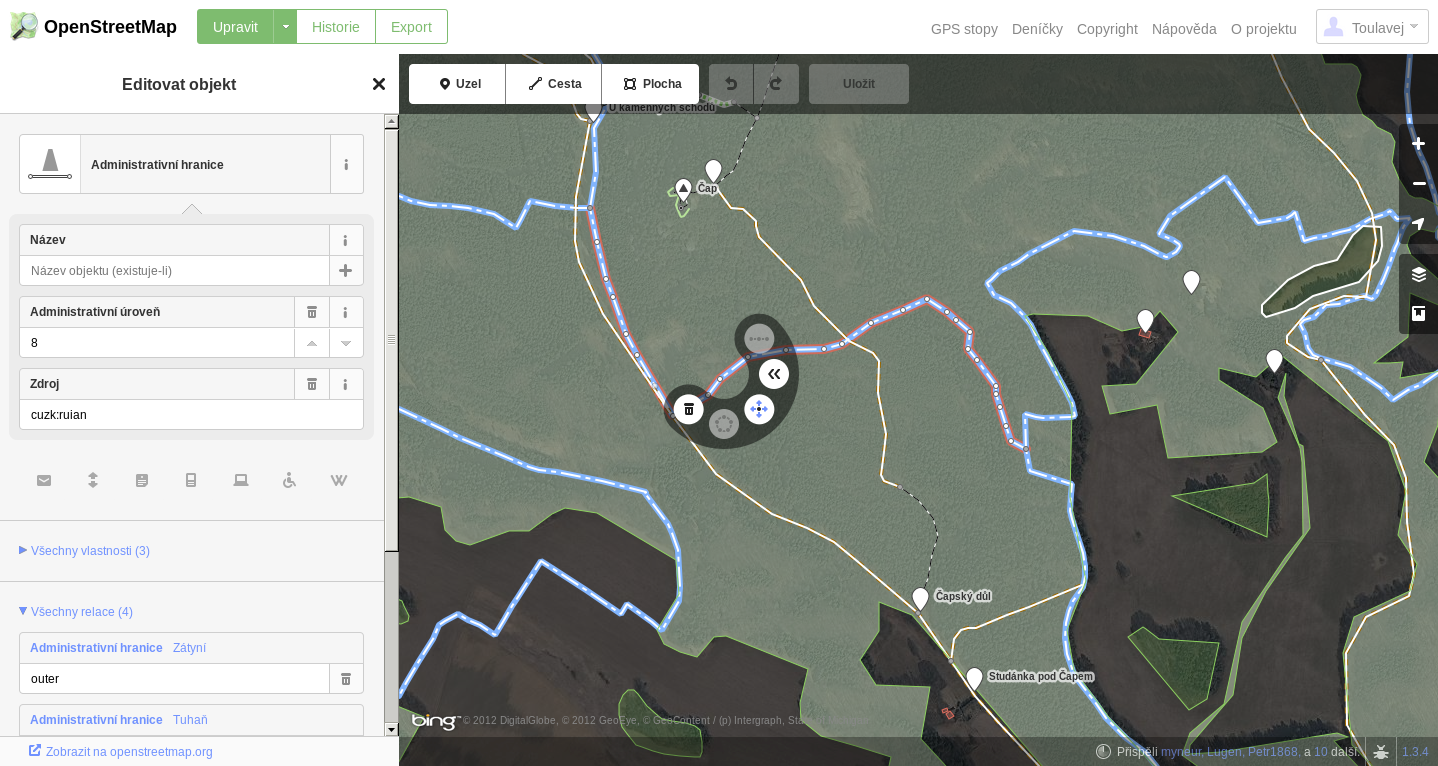
\includegraphics[width=12cm]{obrazky/iD_osm.png}
				\caption{Editor iD na webu OpenStreetMap.org}
				\label{fig:iD_osm}
			\end{center}
		\end{figure}

			\paragraph{} Podle stránek projektu\cite{wiki_iD} program zatím plně nepodporuje prohlížeče Internet Explorer verze 9, 10 a 11. Někteří uživatelé též hlásili zhoršený výkon pro prohlížeč Firefox.

		\subsection{JOSM}
			\paragraph{}JOSM (Java OpenStreetMap Editor) je na Javě založený editor dat OpenStreetMap. Jedná se o desktopovou aplikaci publikovanou pod licencí GPL (General Public License), ze které jsou změny dálkové nahrávány do hlavní databáze OSM. Narozdíl od iD poskytuje JOSM mnohem více možnostní pro manipulaci s daty, což je znát i na jeho uživatelském rozhraní, viz \ref{fig:josm_osm}. Aplikace podporuje čtení GPX souborů buď z pevného disku nebo z databáze OpenStreetMap, editování existujících uzlů, cest, tagů a relací.

                        %%% ML: jediny obrazek se zdrojem, no konecne :-)

		\begin{figure}[!h]
			\begin{center}
				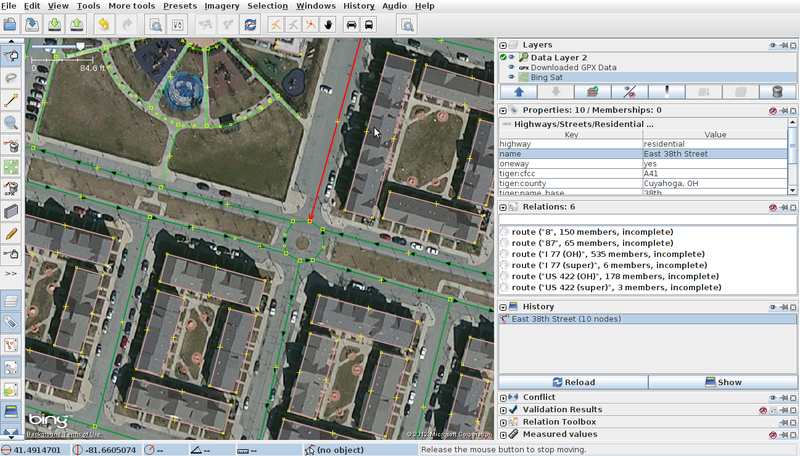
\includegraphics[width=12cm]{obrazky/josm_osm.png}
				\caption{Editor JOSM (zdroj: OSM Wiki\cite{wiki_josm})}
				\label{fig:josm_osm}
			\end{center}
		\end{figure}
			\paragraph{} Výhodou oproti online editorům je možnost pracovat i bez připojení k internetu. Aplikace také poskytuje různá rozšíření, která z ní dělají velmi silný editovací nástroj. Dle informací na OpenStreetMap Wiki\cite{wiki_josm} je práce s tímto editorem jednoduchá. Některé pokročilejší funkce mohou mít složitější ovládání a jejich zvládnutí může zabrat čas.

		\subsection{Merkaator}
			\paragraph{} Editor Merkaator je určen pro Unix, Mac OS i Windows a je distribuován pod licencí GNU GPL v2. Editor je ve stádiu vývoje (dle OpenStreetMap Wiki je dostupná verze 0.18.1 vydaná v červnu 2012), ovšem vývojářská komunita tohoto projektu není příliš aktivní. Aplikace obsahuje prvky, které stojí za povšimnutí. Jedná se například o průhledné zobrazení vrstev, editor stylů zobrazení mapy, přímé připojení k GPS přijímači nebo vykreslení mapy do SVG nebo bitmapového obrázku za použití momentálně užitých stylů. Vzhledem k tomu, že je program ve vývoji, lze některé prvky získat pouze kompilací ze zdrojových souborů, což pro většinu uživatelů není vhodné.

		\begin{figure}[!h]
			\begin{center}
				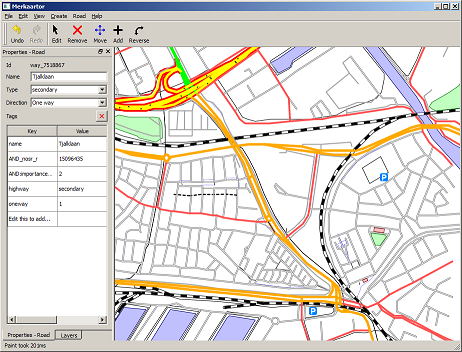
\includegraphics[width=12cm]{obrazky/merkaator_osm.png}
				\caption{Editor Merkaator (zdroj: OSM Wiki\cite{wiki_merkaator})}
			\end{center}
		\end{figure}

		\subsection{Potlatch 2}
			\paragraph{} Stejně jako iD editor je i Potlatch 2 online editor s licencí WTFPL, ale narozdíl od něj je napsán ve Adobe Flash. Jedná se o jednoduchý editor, který není určen pro náročnější uživatele. Potlatch 2 vznikl kompletním přepsáním původního Potlatch, kdy byly přidáno zobrazení WYSIWYG (What You See Is What You Get), jednodušší tagování a autentizace přes OAuth pro zakomponování do jiných stránek při zachování napojení na OpenStreetMap. Z důvodu existence editoru iD není v současnosti aplikace aktivně vyvíjena.

                        %%% ML: zdroj nelze dohledat

		\begin{figure}[!h]
			\begin{center}
				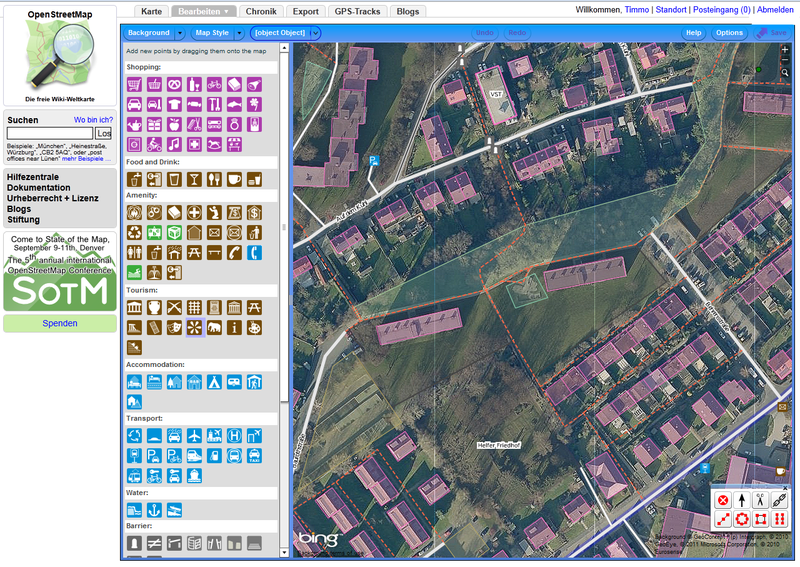
\includegraphics[width=12cm]{obrazky/p2_osm.png}
				\caption{Editor Potlatch 2 (zdroj: OSM Wiki\cite{wiki_p2})}
			\end{center}
		\end{figure}

	\section{Využití dat OSM}
		\paragraph{} Data OpenStreetMap jsou často využívána k tvorbě tématických map, např. z oblasti turistiky. Mapy mohou též sloužit jako podklady do navigací. Řada velkých projektů, např. Foursquare, užívá nebo přechází na mapy OpenStreetMap, protože jsou pro ně výhodnější. Ačkoliv tyto produkty ocení většina uživatelů, dle mého názoru leží větší význam map OpenStreetMap v oblasti humanitární pomoci.
		\paragraph{}V momentě, kdy nějakou část světa zasáhne živelná katastrofa, mohou dobrovolníci z řad uživatelů OpenStreetMap z aktuálních družicových snímků vytvořit novou aktuální mapu postižené oblasti. Toto bylo využito třeba v~roce 2010, kdy bylo Haiti zasaženo zemětřesením, a v současnosti probíhá nové mapování po tajfunu na Filipínách z listopadu 2013. Během prvního týdne od tajfunu bylo editováno víc jak 2 000 000 objektů a do obnovy se zapojilo přes 900 uživatelů. K 11.prosinci 2013 bylo za přispění více jak 1 600 uživatelů zmapováno přes 4,5 milionu objektů \cite{wiki_tajfun}.
		\paragraph{} Aby bylo zajištěno efektivní tvorba, produkce a distribuce map pro postižené oblasti, byla v lednu 2009 vytvořena skupina Humanitarian OpenStreetMap Team \cite{wiki_hot}, která tuto činnost řídí.
	

%%%%%%%%%%%%%%%%%%%%%%%
%%%%% POUŽITÉ TECHNOLOGIE%%%%%
%%%%						      %%%%
%%%							  %%%
%%								     %%
%									 %
\chapter{Použité technologie}
%%%Servery
	\section{Apache HTTP Server}

        %%% ML: v tomto textu michate dohromady specializovany
        %%% software "webovy server" s obecneji vmimanym pojmem
        %%% "server", zkuste tento odstavec prepsat

		\paragraph{} V momentě, kdy je vyvíjena webová aplikace, je nutné mít k~dispozici aplikaci, která by zpracovávala dotazy a posílala odpovědi. Dotazem rozumíme i žádost o přesměrování na jinou stránku. Takovémuto softwaru se říká webový server. Funkce serveru mohou být různé. Velice často obsluhuje webové stránky, ale může sloužit ke skladování dat (datový server) nebo k hraní her (herní server). Při pořizování softwaru je na výběr z několika produktů. Nejčastěji užívaným je Apache HTTP Server, poté je IIS od Microsoftu, nginx od NGINX, Inc. a GWS od Googlu. Protože při vývoji aplikace byl použit server Apache HTTP Server, budou následující řádky věnovány jemu.
		\begin{figure}[!h]
			\begin{center}
				
\includegraphics[width=5cm]{obrazky/apacheLogo.png}
				\caption{Logo projektu Apache HTTP Server}
			\end{center}
		\end{figure}

                %%% ML: "z webove stranky" - mate na mysli "klienta" -
                %%% potom chybi vysvetleni pojmu "server" a "klient"
                %%% (viz odstavec vyse)

		\paragraph{} Apache HTTP Server častěji bývá označován pouze jako Apache. Jeho funkce spočívá v přijímání požadavků z webové stránky, jejich zpracování a vrácení odpovědi. Zpracováním se rozumí např. odeslání statické webové stránky nebo předání požadavku dalším aplikacím. Samotná komunikace je zajištěna přes hypertextový přenosový protokol (HTTP -- HyperText Transfer Protokol). Apache má velké množství modulů, které mohou a nemusí být spuštěny. Pokud jsou zapnuty, rozšiřují možnosti samotného jádra. Při vývoji aplikací je ovšem potřeba, aby na vývojovém a produkčním serveru byly povoleny stejné moduly. V opačném případě může docházet k problémům s funkčností. Běžně užívané moduly jsou např. mod\_rewrite, který slouží k přepisování URL adresy, mod\_php přidávající Apachi podporu pro zpracování PHP skriptů nebo mod\_ssl pro šifrovaná spojení. Ve srovnání s celkovým počtem modulů je toto jen velmi malý vzorek.

                %%% ML: CHYBI zdroj tohoto tvrzeni, musite ho doplnit,
                %%% jinak je to jenom vykrik do tmy

		\paragraph{} Apache je nejrozšířenější webový server -- dle odhadů z června 2013 obsluhovaly servery s Apachem 54,2\% všech aktivních webových stránek. Toto postavení je pravděpodobně způsobeno několika faktory:
		\begin{itemize}
			\item užití Apache License, která umožňuje svobodné užívání softwaru,
			\item veřejně přístupné zdrojové kódy,
			\item rychlost je srovnatelná s komerčními servery a 
			\item podpora všech hlavních operačních systémů.
		\end{itemize}
		
                %%% ML: open chybi zdroj !!!

		\begin{figure}[!h]
			\begin{center}
				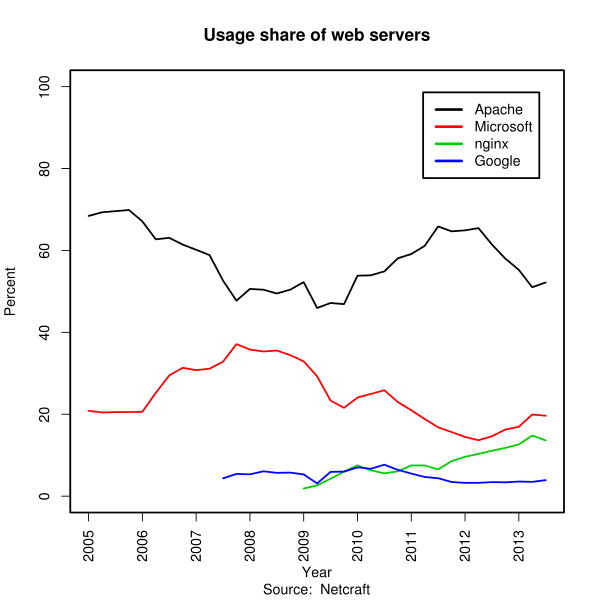
\includegraphics[width=6cm]{obrazky/servers_share.png}
				\caption{Zastoupení jednotlivých serverů}
			\end{center}
		\end{figure}

		\paragraph{} Důvodem pro užití Apache byly přednosti vyjmenované výše -- zejména rychlost a to, že se jedná o svobodný software. Jeho nastavení se sice provádí pomocí textového editoru, to ovšem není taková překážka, protože webové stránky projektu poskytují dostatečnou dokumentaci a v případě problémů není složité dohledat řešení na internetových fórech věnovaných právě serverům. Též svoje sehrálo i to, že Apache obsluhuje školní server geo102.

	\section{Geoserver}
		\paragraph{} V předchozí části bylo uvedeno, že webový server může přesměrovat některé dotazy jiným aplikacím. Dotazy na prostorové informace lze přesměrovat na mapový server. Pokud se pohybujeme v rovině svobodného softwaru, existují dvě možnosti -- Geoserver a UMN MapServer. V komerční sféře lze najít servery od firem Esri, Intergraph a dalších. 

                %%% ML: chybi zdroj

		\begin{figure}[!h]
			\begin{center}
				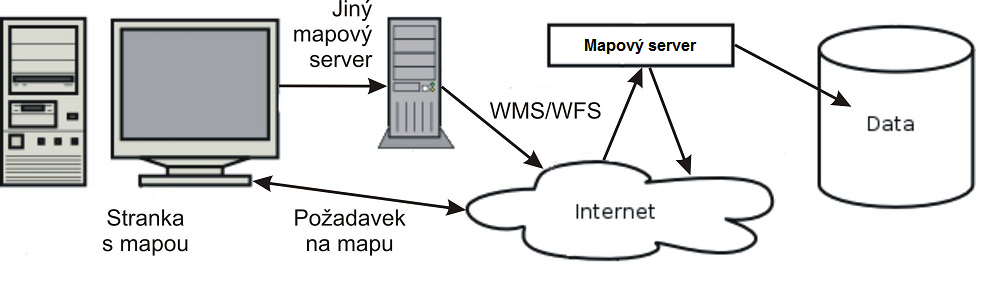
\includegraphics[width=10cm]{obrazky/mapserver.png}
				\caption{Schéma funkce mapového serveru}
				\label{fig:server_schema}
			\end{center}
		\end{figure}
Mapový server podle určitých pravidel vygeneruje obraz požadovaného výřezu mapy, který odešle webovému serveru. Ten ho pak odešle zpátky uživateli. Pravidla pro generování jsou dány parametry, které může a nemusí uživatel zadat. Mezi parametry lze třeba najít požadovaný výstupní formát.

               %%% ML: nejlepsi, proc? tato formulace zavani "flame-war"

               %%% ML: nekomercni? proc? naopak je to vcelku komercne
               %%% vyuzitelne reseni, jiz opraveno na "open source"

               %%% ML: minimalne WMS zkratku by bylo dobre rozepsat...

		\paragraph{} Geoserver je v současné době asi nejlepší open source řešení\cite{vorlicek} s  podporou všech běžně užívaných webových služeb. Aplikace podporuje velké množství vstupních a výstupních formátů. Vstupem může být například PostGIS databáze, Esri Shapefile, GeoTIFF či WMS služba. Výstup může být například ve formátu PNG, PDF, JPEG, KML, CSV nebo JSON.  Geoserver je napsán v Javě a pro jeho nastavení a správu se používá webové rozhraní, které je normálně dostupné na portu 8080, ale tento port může být změněn. Zde lze nastavit poskytované vrstvy a služby. Správa uživatelů a uživatelských rolí se provádí také zde. 
		\begin{figure}[!h]
			\begin{center}
				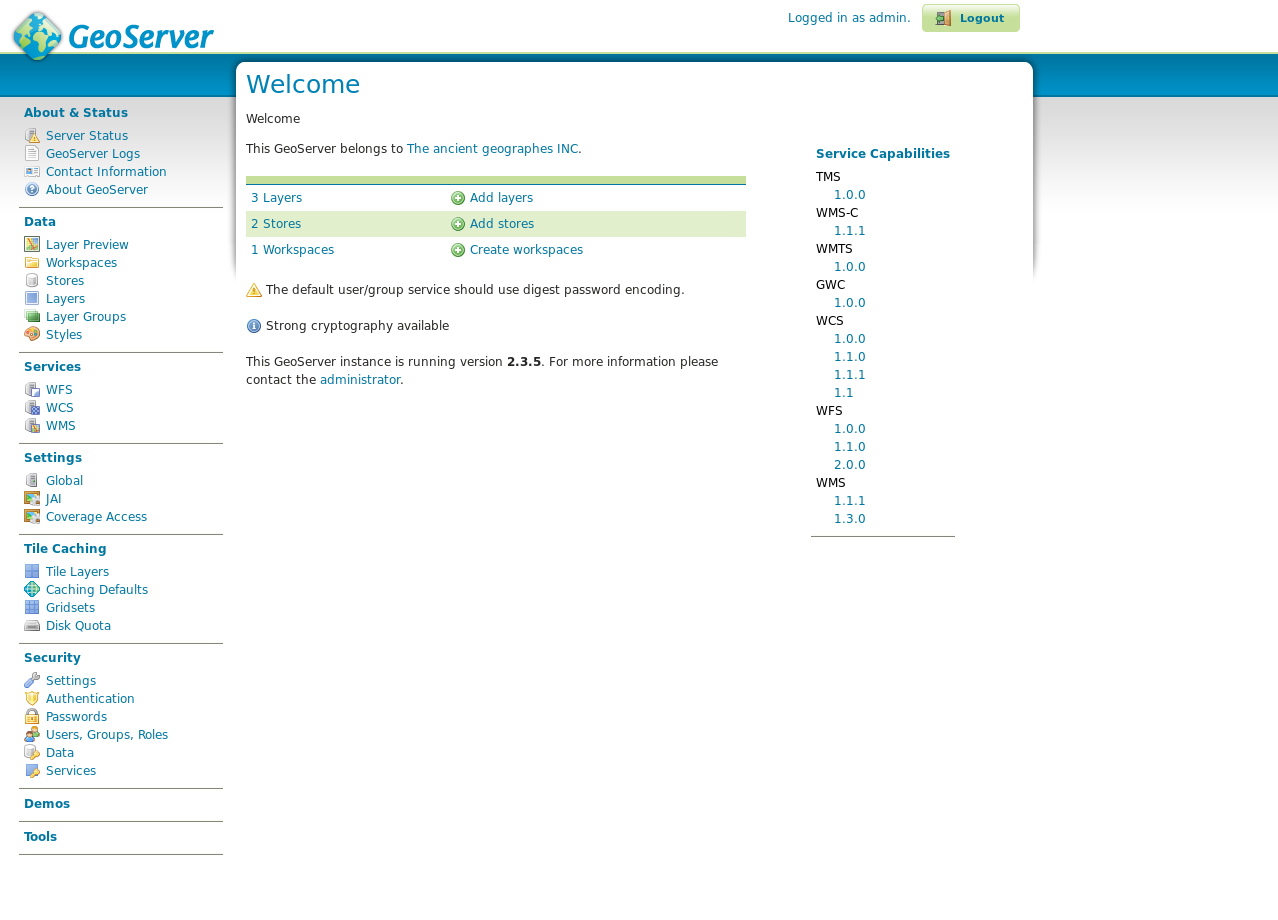
\includegraphics[width=10cm]{obrazky/geoserver.png}
				\caption{Uživatelské rozhraní Geoserveru}
			\end{center}
		\end{figure}

                %%% ML: "Jedná se typ XML (eXtended Markup Language)."
                %%% neexistuje "typ" xml, SDL je odvozen ci zalozen na
                %%% XML

		\paragraph{}Pro nastavení vzhledu publikovaných vrstev se používá SLD (Styled Layer Descriptor) schéma. Jedná se typ XML (eXtended Markup Language). Pravidla lze zapsat do textového pole, což není moc pohodlné. Naštěstí Geoserver poskytuje možnost importovat pravidla  vytvořená v jiném programu. Takto lze úspěšně použít Quantum GIS\cite{qgis} či AtlasStyler\cite{atlas} pro tvorbu vzhledu prvků.

                %%% ML: co je WMS-T a proc to bude potreba, vysvetlit
                %%% ci uvest odkaz na kapitolu, kde to bude vysvetleno

                %%% ML: proc nemohl byt pouzit MapServer, vysvetlit

		\paragraph{} Výběr Geoserveru byl dán zejména snahou využít svobodný software. Před začátkem tvorby se předpokládalo, že aplikace bude potřebovat WFS-T službu. MapServer tedy nemohl být použit a Geoserver se jevil jako dobrá volba. V jeho prospěch také hrálo uživatelské rozhraní pro nastavení a publikování vrstev, protože MapServer se nastavuje pomocí konfiguračních souborů.

%%%Databáze
	\section{PostgreSQL}

        %%% ML: "bere data" - to snad ne ;-) PREPISTE TO

        %%% ML: samotny soubor? neco jako souborove orientovany format
        %%% jako napr. Esri Shapefile

        %%% ML: vyuziti jednotlivych souboru? jakych ?


        %%% ML: "PostgreSQL nabízí širší škálu funkcí" --- nezminujete
        %%% se vubec o PostGISu, aha, je zminka v dalsim odstavci

		\paragraph{} Na obrázku \ref{fig:server_schema} je zobrazeno, že si mapový server bere data. Data jsou uložena buď v samostatném souboru nebo v databázi. Pro potřeby webových aplikací se spíše užívají databáze, ačkoliv využití jednotlivých souborů také není vyloučeno. Mnoho webových aplikací používá relační databázi MySQL, ale z hlediska vhodnosti pro tuto aplikaci byla zvolena jiná relační databáze -- PostgreSQL. Ačkoliv MySQL má podporu pro prostorová data, PostgreSQL nabízí širší škálu funkcí. Navíc existují pro PostgreSQL programy, které usnadňují import dat OpenStreetMap. V neposlední řadě k této volbě přispěl i fakt, že projekt OpenStreetMap používá PostgreSQL.
		\begin{figure}[!h]
			\begin{center}
				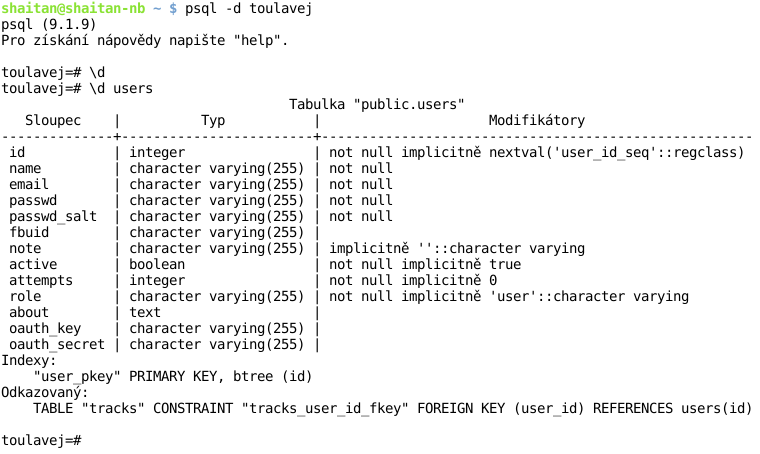
\includegraphics[width=10cm]{obrazky/psql.png}
				\caption{Terminál s aplikací psql}
				\label{fig:psql}
			\end{center}
		\end{figure}


                %%% ML: nezapomente na kontrolu pravopisu, na rade
                %%% mist jsem opravil chyby jako "standart" a dalsi

                %%% ML: "hashích" ??? to neni odborny termin

		\paragraph{}PostgreSQL je databázový systém napsaný v jazyce C. Kromě Linuxu je možné s ním pracovat i na počítačích s operačními systémy Windows, Mac OS X, Solaris aj. PostgreSQL je licencován pod PostgreSQL License, která je podobná licenci MIT.  Implementace SQL v PostgreSQL  odpovídá standardu ANSI--SQL:2008\cite{postgresql} a také obsahuje většinu ze standardu SQL:2011\cite{wiki_postgresql}. Systém podporuje použití primárních (PRIMARY) a cizích klíčů (FOREIGN KEYS), triggerů, podmínek UNIQUE a NOT NULL. Indexy mohou být uloženy v B-stromech, R-stromech, hashích nebo GiST (Generalized search tree) vyhledávacích stromech. Současná stabilní verze PostgreSQL má číslo 9.3.2. PostgreSQL se dá přizpůsobit podle potřeb uživatelů, díky čemuž vznikly různá rozšíření. 
		\begin{figure}[!h]
			\begin{center}
				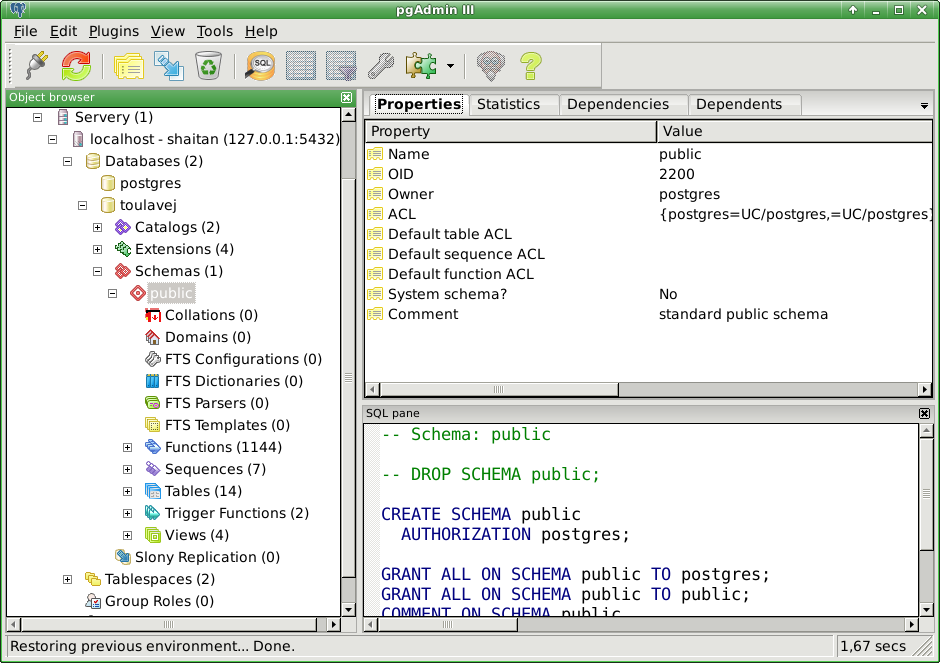
\includegraphics[width=8cm]{obrazky/pgadmin3.png}
				\caption{Desktopová aplikace pgAdmin III}
				\label{fig:pgadmin}
			\end{center}
		\end{figure}
		\paragraph{}Z existujících rozšíření mají spojitost s vytvářeným projektem dva balíky. Prvním z nich je PostGIS, který poskytuje podporu pro geografická data. Tento balík přidává do systému geometrii prvků a funkce pro práci s nimi. Druhým rozšířením je pgRouting, který poskytuje funkce pro síťové analýzy. Oba výše zmíněné projekty jsou šířeny pod licencí GNU GPL.
		\begin{figure}[!h]
			\begin{center}
				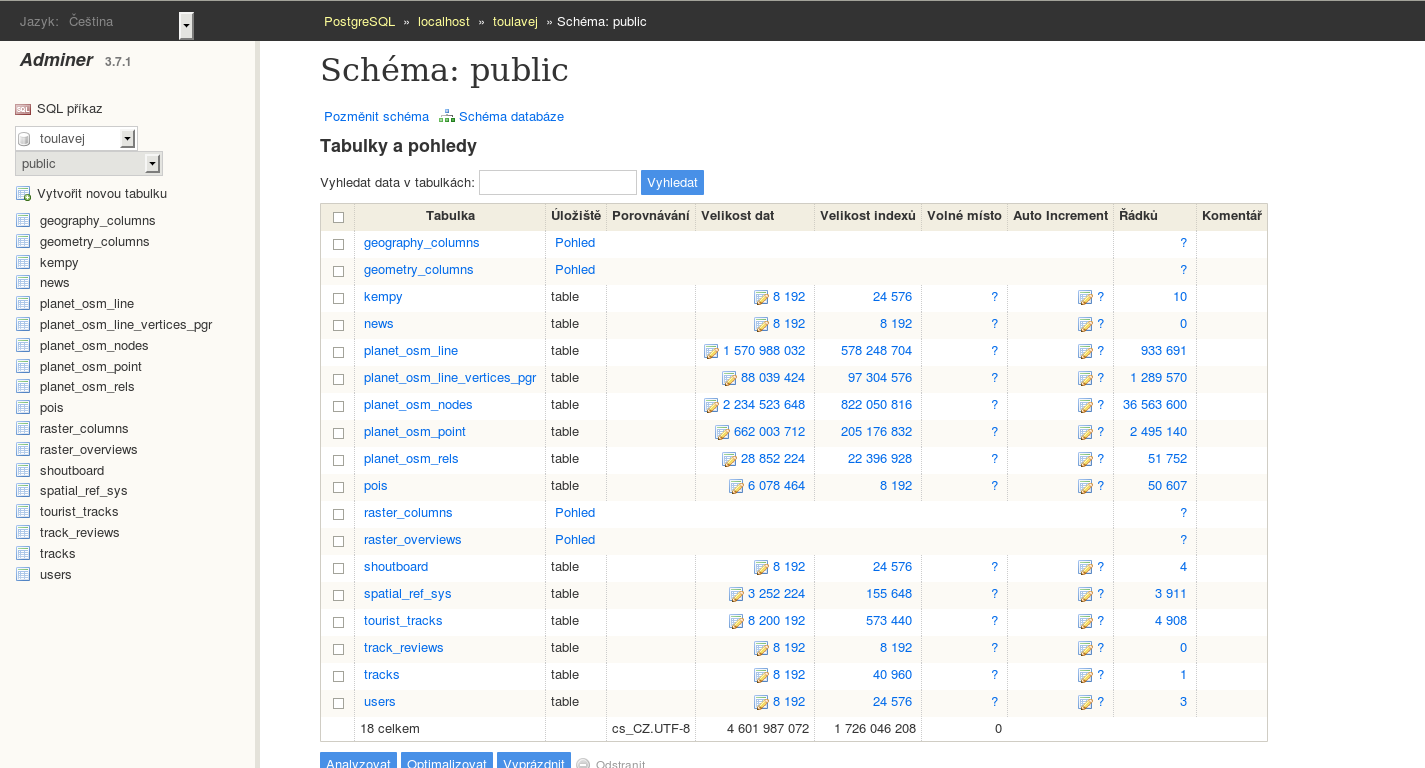
\includegraphics[width=10cm]{obrazky/adminer.png}
				\caption{Webová aplikace Adminer}
				\label{fig:adminer}
			\end{center}
		\end{figure}			

                %%% ML: co je shell, neni vysvetleno, ctenar bez
                %%% hlubsi zkusenosti asi bude zmaten

		\paragraph{}Samotná databáze musí být nějak spravována. V operačním systému Linux lze použít program psql \ref{fig:psql} využívající příkazový řádek, grafické rozhraní pgAdmin III \ref{fig:pgadmin} nebo PHP program Adminer \ref{fig:adminer}. Každá z uvedených variant má své výhody. Pro práci s databází v rámci skriptu napsaného pro shell najde uplatnění právě příkazový řádek, pro práci na vzdáleném počítači lze využít Adminer, který se spouští přes webové rozhraní a pro práci na lokálním počítači se dá použít pgAdmin3.




%%%Programovací jazyky
	\section{PHP}
		\paragraph{} Pro zpracování dynamických požadavků na serveru je potřeba použít nějaký programovací jazyk. Tyto jazyky bývají označovány jako server--side. Patří mezi ně ASP, ASP.NET, C (při použití CGI rozhraní), Java, Perl, PHP a další. V této aplikaci je použit poslední jmenovaný jazyk. PHP (název je rekurzivní zkratka -- PHP: Hypertext Preprocessor) je určený především pro tvorbu dynamických webových aplikací, ale lze ho využít i pro tvorbu konzolových a desktopových aplikací. PHP je platformně nezávislý programovací jazyk, který lze rozšířit mnoha knihovnami. Pro tvorbu webových aplikací se PHP nejčastěji užívá se serverem Apache a databází MySQL. Tyto tři aplikace lze stáhnout v jednom balíku, který je podle platformy označován zkratkou LAMP(pro Linux) nebo WAMP(pro Windows).

                %%% ML: kde jsou pouzivany starsi verze, neni prilis jasne

		\paragraph{} Současná verze PHP je 5.5, která byla vydána k 20.6.2013, ale používány jsou i starší verze jazyka. Při vývoji se užívá buď čisté PHP a nebo v podobě frameworků, které mají už naprogramované často užívané prvky. Tímto je usnadněna práce vývojáře, protože se může plně věnovat úkolu, který řeší. Frameworky také zajišťují větší bezpečnost, protože úkony jako přístup do databáze jsou již ošetřeny proti chybám a programátorovi stačí zavolat potřebnou funkci. Argumentem proti frameworkům je nižší rychlost zpracování požadavků a potřeba se naučit práci s ním. Pokud se framework používá na větších projektech, či počet projektů, kde je užit, je větší, tak čas, který práce s frameworkem ušetří, je větší než doba, která je potřeba k zvládnutí práce s ním.
		\subsection{Framework Nette}
			\paragraph{} Jedná se o open source framework českého původu, který je určený pro tvorbu aplikací v PHP 5.  Autorem je David Grudl, ale v současné době se o vývoj stará organizace Nette Foundation. K 11.12.2013 byla uvolněna ke stažení verze 2.1.0 RC3, která je pod licencí NewBSD a GNU GPL.  
			\paragraph{} Hlavním cílem je tvorba bezpečných aplikací. Mimo jiné je zde implementována ochrana před Cross-site scripting (XSS), která ošetřuje data z~uživatelských vstupů a zabraňuje tak, aby útočník podstrčil svůj vlastní kód. Ačkoliv je otázka bezpečnosti první v seznamu výhod, není zdaleka poslední. Velmi silným argumentem pro jeho užití je snadné tvoření formulářů. Nette formuláře poskytují velké množství validačních pravidel. Automaticky generovaný validační javascriptový kód může být brán jako bonus.

                        %%% ML: Laděnka? vysvetlit

			\paragraph{} Při práci s Nette je možné ale ne nutné nastavit vývojový nebo produkční režim. Výhodou nastavení takovéhoto rozdělení je možnost nakopírování aplikace z vývojového serveru na produkční a aplikace podle adresy serveru bere požadované parametry, např. jméno databáze, přihlašovací jméno a  heslo a další. Ve vývojovém prostředí je pak dostupná Laděnka, která pomáhá v debugování celé aplikace.
			\paragraph{} Velkou výhodou je, že v českém prostředí má Nette aktivní komunitu uživatelů, kteří kromě tvorby mnoha komponent pořádají i pravidelné srazy uživatelů.  Uživatelé a vývojáři frameworku jsou též aktivní na fórech, kde lze řešit problémy v aplikacích a chyby ve frameworku Nette.
			\subsubsection*{Návrhový vzor}
				\paragraph{} Návrhovým vzorem rozumíme architekturu aplikace. Jinými slovy se jedná o určité části (vrstvy) aplikace, které zajišťují různé funkcionality. V Nette se užívá architektura MVP (Model -- View -- Presenter).

                                %%% ML: zkuste odstavec prepsat (model)

				\paragraph{Model} je označení pro vrstvu, která se stará o propojení s databází. Vkládání, změna, výpis i mazání dat jsou akce, které jsou záležitostí modelu. Model má nadefinované své funkce, kterými obsluhuje databázi. Okolí komunikuje s modelem pomocí pevně daného rozhraní. V Nette je tato vrstva implementována v knihovně Nette Database. Pro větší přehlednost se vytvářejí funkce, které vypisují potřebná data. Tím nedochází k pokládání dotazů ve zdrojovém kódu Presenterů.

                                %%% ML: "V Nette se o tuto funkci
                                %%% starají šablony napsané latte."
                                %%% ???

                                %%% ML: chybi vysvetleni pojmu "sablona"

				\paragraph{View} je vrstva, která vykresluje výsledek zadaného požadavku. V Nette se o tuto funkci starají šablony napsané latte. Latte je šablonovací systém napsaný v PHP, ovšem díky němu je psaní šablon jednodušší, přehlednější a bezpečnější než kdybychom je psali v čistém PHP.
				\paragraph{Presenter} je spojovací vrstva, která předává data z modelu do view k vykreslení a akce z view zpracovává a předává modelu. Presenter je ekvivalentem Controlleru z architektury MVC s tím rozdílem, že Controller zpracovává i některé události uživatelského rozhraní.

	\section{JavaScript} %openLayers, Leaflet, jQuery a další
		\paragraph{} Každá webová stránka občas potřebuje zobrazit dynamický obsah, který bude okamžitě reagovat na uživatelské vstupy. V aplikacích vytvořených v programovacím jazyce Java zajišťuje jak práci na serveru, tak interakci na klientském počítači. Jazyk PHP má ke zpracování uživatelských vstupů trochu jiný přístup. PHP nedokáže dynamicky měnit obsah stránky bez nového načtení této stránky. Tento nedostatek jazyka se dá odstranit užitím jazyka JavaScript.

                %%% ML: zdroj?

		\begin{figure}[!h]
			\begin{center}
				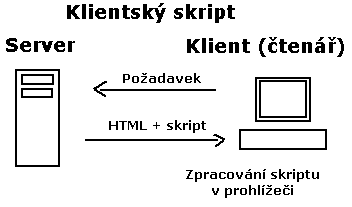
\includegraphics[width=5cm]{obrazky/klient_skript.png}
				\caption{Princip klientského skriptu, např. JavaScriptu}
				\label{fig:client}
			\end{center}
		\end{figure}	
		\paragraph{} JavaScript byl vyvíjen jako jazyk Mocha ve firmě Netscape pro potřeby prohlížeče Navigator, ve kterém se objevil jako LiveScript. JavaScript je též znám jako ECMAScript. Díky svému jménu bývá často chybně spojován s programovacím jazykem Java. Oba jazyky mají podobnou syntax, ale to mají i s jinými jazyky, např. PHP nebo C++. Každý z jazyků vytvořila jiná firma -- JavaScript byl vytvořen v Netscapu a Java v Sun Microsystems. JavaScript je hojně užíván pro tvorbu dynamického obsahu webových stránek, a proto se občas označuje za programovací jazyk webových stránek, ačkoliv se pro tvorbu internetových stránek používá jazyk HTML.

                %%% ML: konec odstavce : "a ten pouze nahrát", čtenař
                %%% se
                %%% bude ptat, "nahrat kam", a proc "pouze", cela veta
                %%% by chtela
                %%% prepsat

		\paragraph{} Využití JavaScriptu je zejména v tvorbě dynamických prvků na webových stránkách. JavaScritpový kód je posílán ke klientovi na počítač, kde je zpracován\label{fig:client} interpreterem, který je součástí každého moderního prohlížeče. JavaScript je možné zapsat do HTML souboru pomocí tagů \htmlTag{script}. Pokud se jedná o delší skript, je lepší ho dát do zvláštního souboru a ten pouze nahrát.
		\paragraph{AJAX} Asynchronní JavaScript A XML je jedno z běžných užití Java\-Scriptu, které umožňuje posílat XML dotazy na server bez znovunačtení stránky. Server tento dotaz obslouží, vrátí výsledek a ten se zobrazí na stránce. Tato technika obnovování stránky si získala oblibu díky službám společnosti Google. Tento přístup je též užíván v knihovnách jako jsou OpenLayers nebo Leaflet pro získání a zobrazení mapy.

		\begin{figure}[!h]
			\begin{center}
				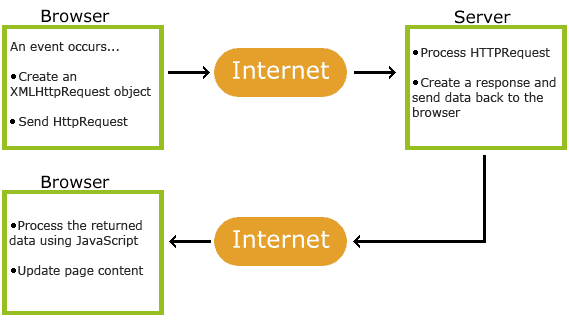
\includegraphics[width=5cm]{obrazky/ajax.png}
				\caption{Princip fungování AJAXu}
				\label{fig:ajax}
			\end{center}
		\end{figure}	

		\subsection{OpenLayers} %v2 v3
			\paragraph{} JavaScript lze využít pro tvorbu mnoha dynamických prvků stránek, ale pro složitější prvky je vhodnější použít nějaké existující nástroje. Pro tvorbu mapových aplikací existuje několik knihoven, které poskytují  API  pro usnadnění práce. Jednou z takových knihoven je OpenLayers.
			\paragraph{} Jedná se o knihovnu s otevřeným kódem, která je šířena pod licencí BSD. OpenLayers byly vytvořeny firmou MetaCarta mezi roky 2005 a 2006 a od listopadu 2007 je o jejich vývoj stará Open Source Geospatial Foundation. Aktuální stabilní verze je 2.13.1, ale souběžně s OpenLayers verzí 2 se vyvíjí i verze 3, která je dostupná ve verzi 3.0.0-beta.1. OpenLayers~3 vzniká přepisování původní verze a začleněním nových technologií, které umožňují využití HTML5 a CSS3. Vytvoření mapy s novou verzí je oproti minulé verzi rychleší a výsledný kód je přehlednější.
			\paragraph{}OpenLayers jsou schopné zobrazit velké množství formátů -- od rastrových dat ve formátu JPEF nebo PNG až po vektorová data GeoJSON či GML. Data lze připojit přímo z disku nebo je lze získat pomocí WMS nebo WFS služby. Velkým plus této knihovny je velice dobře zpracovaná dokumentace a vzorové příklady, které pomohou při tvorbě mapové aplikace. 
		\subsection{Leaflet}
			\paragraph{} Druhou knihovnou, kterou lze užít na tvorbu webové mapové aplikace, je javascriptová knihovna Leaflet. Jedná se o moderní knihovnu srovnatelnou s OpenLayers 3. Leaflet se dá též použít pro zobrazení aplikace na mobilních zařízeních. Stejně jako OpenLayers 3 je i Leaflet stále ve vývoji (od listopadu 2013 je dostupná verze 0.7.1), takže některé prvky stále nejsou plně funkční či chybí úplně. Dobře zdokumentované API a návody pro začátečníky jsou velice dobrým pomocníkem při tvorbě map, stejně tak i různé zásuvné moduly, které vytvořili členové komunity.
		\paragraph{} Ačkoliv Leaflet a OpenLayers 3 jsou modernější, pro vývoj aplikace byla použita stávající verze OpenLayers v2. Původně zvažovaný Leaflet byl zamítnut kvůli problémům s připojením vektorových vrstev a kvůli tomu, že se stále jedná o vývojovou verzi. Ze stejného důvodu nebyla použita ani knihovna OpenLayers 3.

                %%% ML: najdete mene zavadejici nazev pro tuto
                %%% kapitolu...

	\section{Grafika}

        %%% ML: "grafika uzivatelskeho rozhrani" slysim poprve, zkuste
        %%% spise operovat s pojmem "design" nebo navrh UI

        %%% ML: "tvorba grafiky" ??? design ...

		\paragraph{} Důležitým prvkem webové stránky je její grafické provedení, protože špatně vytvořený vzhled webu může odradit potenciální zákazníky. Důležitost grafiky uživatelského rozhraní dokazuje i to, že dost firem vyvíjejících webové stránky a aplikace má ve svém týmu člověka, který se věnuje zejména tvorbě grafiky.

                %%% ML: prvku ceho?

		\paragraph{} Hlavním nástrojem pro určení pozice, barvy, velikosti a chování prvků při zmenšení/zvětšení okna jsou \textit{kaskádové styly} (Cascading style sheets) označované zkratkou CSS. Vzhled stránky může být definován v sekci \htmlTag{head} souboru s HTML kódem stránky nebo pomocí vlastnosti \textit{style} přímo u prvku, ale častěji se kvůli přehlednosti využívá zapsání do samostatného souboru, který se do HTML dokumentu importuje podobně, jako javascriptový soubor. Kaskádovými styly lze modifikovat vzhled všech HTML prvků. 

                %%% ML: "zapsani" ??

                %%% ML: "První možností je užítí na všechny prvky
                %%% stejného typu" - zkuste prepsat...

		\paragraph{} Kaskádové styly mají tři úrovně zapsání. První možností je užítí na všechny prvky stejného typu, např. pro nastavení stejného vzhledu všech nadpisů \htmlTag{h1}. Pro definování vzhledu jen určitých prvků je možné použít třídy. V HTML tagu se pomocí vlastnosti \textit{class} zavolá požadovaný styl. Pokud v dokumentu existují unikátí prvky, tak lze k jejich nastylování použít id. Volání se provádí v HTML tagu pomocí vlastnosti \textit{id}.

                %%% ML: "vrstvit" nezni moc pekne ...

		\paragraph{} Aby bylo možno dosáhnout požadovaného výsledku, umožňují kaskádové styly vrstvit jednotlivá pravidla, jak je zobrazeno na příkladu webu Seznam.cz\ref{fig:seznam}. Ne všechny prohlížeče zobrazují všechny stránky stejně. U Microsoft Internet Exploreru je interpretace CSS stylů odlišná od jiných prohlížečů, což vede vývojáře k vytváření speciálních pravidel pro tento prohlížeč.
		\begin{figure}[!h]
			\begin{center}
				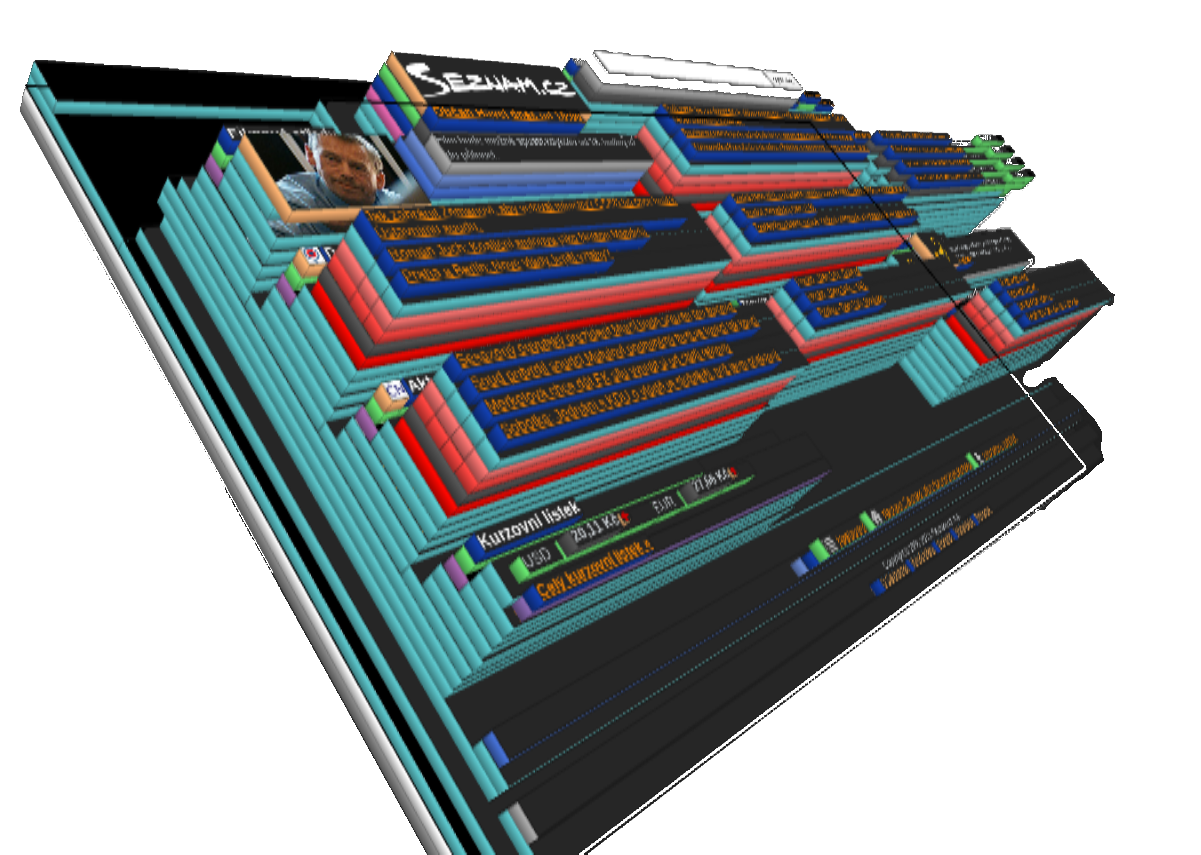
\includegraphics[width=12cm]{obrazky/css_vrstvy.png}
				\caption{Zobrazení CSS vrstev webu Seznam.cz}
				\label{fig:seznam}
			\end{center}
		\end{figure}	

                %%% ML: odkaz na Twitter, poznamka pod carou, vysvetleni...

		\paragraph{} Pro usnadnění práce vývojářů vznikly různé šablony a frameworky. V~pří\-padě vyvíjené aplikace byl použit Bootstrap (v2.2.2) -- framework s otevřeným zdrojovým kódem vytvořený pro Twitter v polovině roku 2010. Ve verzi 2 byla přidána podpora responsivního designu, což zaručuje správné zobrazení aplikace i na mobilních zařízeních. Začátkem prosince 2013 byl vydán Bootstrap ve verzi 3.0.3, která má v základu nastavený responzivní design a bere ohled na mobilní zařízení.
%%%%%%%%%%%%%%%%%%%%%%%
%%%%% 	VÝVOJ APLIKACE	   %%%%%
%%%%						      %%%%
%%%							  %%%
%%								     %%
%									 %
\chapter{Vývoj aplikace}
		\section{Databáze}
			\subsection{Datový model}
				\paragraph{} Databáze je důležitým prvkem aplikace Toulavej -- jsou zde uloženi registrovaní uživatelé, příspěvky v diskuzi a další data včetně dat OpenStreetMap. Databáze byla vytvářena postupně podle toho, které tabulky byly potřeba. Všechny tabulky a sloupce jsou pojmenovány anglicky. V obrázku \ref{fig:db} jsou vidět tabulky a vztahy mezi nimi. V schématu nejsou zobrazeny tabulky vzniklé importem dat planet\_osm a tabulky rozšíření PostGIS. 
				\paragraph{}Tabulka \textit{news} je určena pro ukládání událostí, které jsou zveřejňovány jako novinky. Zde se evidují pouze položky \textbf{id} jako primární klíč, \textbf{user\_id} jako cizí klíč na tabulku \textit{users}, \textbf{note} s novinkou a čas vytvoření(\textbf{created}).
				\paragraph{}Další v pořadí je tabulka \textit{pois} odvozená od bodové vrstvy dat OpenStreetMap. Vznikla vybráním bodů, které by mohly být pro uživatele nějakým způsobem zajímavé. Hlavní sloupce jsou \textbf{osm\_id} pro primární klíč a \textbf{way} pro geometrii. Sloupce \textbf{amenity, historic, leisure, man\_made, name, natural, religion, shop a tourism} obsahují informaci o typu prvku. Zde je velice častý výskyt hodnoty NULL. Sloupec \textbf{tags} užívá rozšíření hstore a jsou v něm uvedeny další informace.
		\begin{figure}[!h]
			\begin{center}
				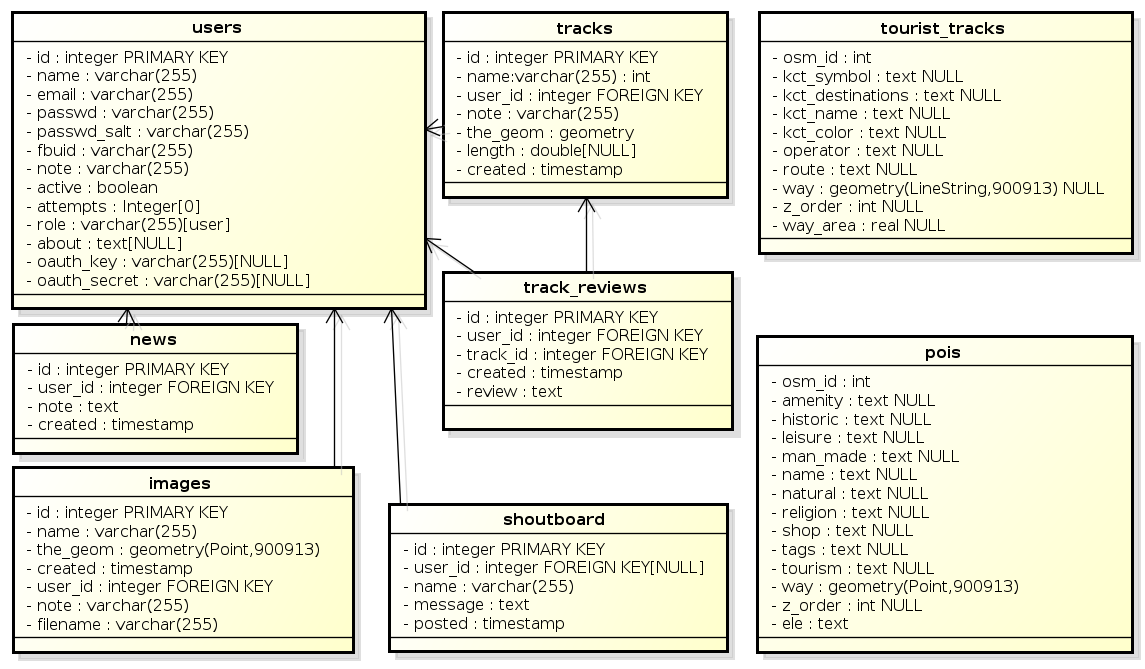
\includegraphics[width=13cm]{obrazky/datovy_model.png}
				\caption{Datový model databáze projektu Toulavej}
				\label{fig:db}
			\end{center}
		\end{figure}
                        \paragraph{} Další tabulkou odvozenou z liniové vrstvy dat OpenStreetMap jsou \textit{tourist\_tracks}. Stejně jako \textit{pois} nese sloupec s primárním klíčem označení \textbf{osm\_id}. Sloupec \textbf{kct\_color} určuje barvu turistické stezky bez ohledu na druh značky. Ten je zohledněn v \textbf{kct\_symbol}. Možné cíle trasy(pokud jsou uvedeny) udává \textbf{kct\_destinations}. Pokud má trasa nějaké jméno, je uvedeno v \textbf{kct\_name}. Zřizovatel trasy je uveden v \textbf{operator}. V poli \textbf{route} je uveden typ cesty. Geometrii lze nalézt ve sloupci \textbf{way}. \textbf{way\_area} určuje plochu ohraničenou uzavřeným liniovým prvkem.
			\paragraph{} Tabulka \textit{tracks} slouží k ukládání uživateli vloženými trasami. Na uživatele, který příspěvek vložil, odkazuje po \textbf{user\_id}. Geometrii lze najít v \textbf{the\_geom} a délka je v \textbf{length}. Do pole \textbf{note} se vkládají poznámky či možné cíle trasy. \textbf{Id} určuje primární klíč a \textbf{created} je čas uložení do databáze. Na tuto tabulku se váže přes cizí klíč \textbf{track\_id} tabulka \textit{track\_reviews}, která slouží k ukládání komentářů a hodnocení k cestám. \textit{Track\_reviews} se váží přes \textbf{user\_id} na tabulku \textit{users}. Dále je zde samotný text(\textbf{review}) a časová známka, kdy byl příspěvek vložen(\textbf{created}).
			\paragraph{}Tabulka \textit{users} slouží k ukládání dat o registrovaných uživatelích. Pole \textbf{id} je primární klíč, které má výchozí hodnotu nastavenou na další číslo v pořadí. Pole \textbf{name} je jméno, které zadává uživatel při registraci nebo které se vezme z profilu na Facebooku. Toto jméno lze v nastavení změnit. Tabulka obsahuje pole s emailem, který spolu s heslem slouží k přihlášení do aplikace. Pokud je uživatel připojen přes Facebook, uloží se jeho identifikace na Facebooku do pole \textbf{fbuid}. Pole \textbf{active} slouží k případnému znemožnění přihlášení uživatele a pole \textbf{attempts} ukazuje počet neúspěšných pokusů o přihlášení. Pokud dosáhne jejich počet určitého množství, tak se účet zablokuje. Sloupec \textbf{role} udává, jaká práva má daný uživatel. V systému jsou tři typy rolí (guest, user a admin) ale pouze user a admin se ukládají do tabulky. Volitelné pole \textbf{about} umožňuje uživateli napsat o sobě pár informací a \textbf{note} slouží k zapsání poznámky pro administrátora. Sloupce \textbf{oauth\_key} a \textbf{oauth\_secret} jsou určeny pro přihlašování do OpenStreetMap.
			\paragraph{}Tabulky, které jsou doplňovány, jsou prázdé a jediné záznamy, které se vkládaly při tvorbě, jsou administrátorovy uživatelské informace.

			\subsection{Naplnění databáze}
				\paragraph{} Před zahájením samotného naplnění databáze bylo potřeba aktivovat rozšíření. Jednalo se o \textit{PostGIS} rozšíření pro práci s prostorovými daty, \textit{PgRouting} pro plánované vyhledávání cest mezi zadanými body a \textit{hstore} pro usnadnění práce s daty ve sloupcích \textbf{tags}. Na tyto úkony je potřeba administrátorský přístup, takže potřebné modifikace v databázi na serveru \textit{geo102} provedl Ing. Landa.
				\paragraph{} V momentě, kdy byla databáze připravena, bylo možné vytvořit tabulky a nahrát data. Pro získání dat OpenStreetMap byla použita internetová stránka \url{http://download.geofabrik.de/europe/czech-republic.html}, kde jsou data Planet.osm rozdělena podle kontinentů a zemí. Tato data jsou každý den aktualizována. Nejjednodušším způsobem, jak nahrát data do databáze, je pomocí konzolové aplikace \textit{osm2pgsql}. Při importu dat může dojít k tomu, že užívaný počítač nemí potřebnou operační paměť. Program \textit{osm2pgsql} tento problém řeší pomocí tzv. \textit{slim modu}, ve kterém jsou využita dočasná úložiště. Ta zmenší velikost potřebné operační paměti. Databáze České republiky zabírá zhruba 4 GB paměti, ovšem ne všechna data jsou pro projekt potřebná. V případě turistických stezek byla potřebná data uložena do speciální tabulky, protože jejich výběr z původní tabulky za pomoci SELECTu nebo VIEW byl zdlouhavý. Ze stejného důvodu byly vybrány i zájmové body. Při prvním nahrání databáze vznikl problém se získáním údajů z pole \textbf{tags}. V dokumentaci \textit{PostgreSQL} na stránkách aplikace byl uveden příklad, jak je získat. Tento problém poté odpadl s aktivací rozšíření \textit{hstore}. Kvůli výsledné velikosti databázi je zvažováno, že po zprovoznění vyhledávání cest budou tabulky s nepotřebnými daty odstraněny. Aby se k datům dalo přistupovat z aplikace, bylo potřeba správně nastavit práva.
				\paragraph{} V neposlední řadě bylo potřeba doplnit tabulky, které nevznikají z dat OpenStreetMap:
					\begin{itemize}
						\item news -- novinky generované při některých akcích či zadané administrátorem
						\item  shoutboard -- tabulka pro diskuzi
						\item  track\_reviews -- komentáře a články k trati
						\item  tracks -- uživateli zadané trasy
						\item users -- informace o uživatelích včetně jejich přihlašovacích údajů
					\end{itemize}
Většina těchto tabulek neobsahuje prostorová data, jenom tabulka \textit{tracks} má prostorovou složku.
			\subsection{Aktualizace databáze}
				\paragraph{} Protože se data OpenStreetMap neustále vyvíjí a zpřesňují, je potřeba je jednou za čas aktualizovat. Vzhledem k tomu, že se jedná o časově náročnou činnost (import dat OpenStreetMap trvá na serveru kolem 1 hodiny), byl vytvořen skript, který provede potřebné kroky automaticky poté, co je předchozí úkol hotov. Skript postupuje v následujících krocích.
		\begin{enumerate}
			\item Stáhne aktuální data pomocí příkazu \textit{wget}  z \url{http://download.geofabrik.de/europe/czech-republic-latest.osm.bz2}.
			\item Rozbalí data pomocí programu \textit{bunzip2}.
			\item Za užití \textit{osm2pgsql} s parametry \textit{ -\--slim  -\--cache--strategy dense -\--hstore --d vorlichr\_dp} importuje data do databáze.
			\item Program psql vytvoří tabulku \textit{tourist\_tracks} podle SELECTu ze souboru \textit{hiking\_routes.sql}.
			\item Ze souboru \textit{pois.sql} použije \textit{psql} dotaz na vytvoření tabulky \textit{pois}.
			\item Spustí se skript, který správně nastaví přístupy k databázi.
			\item V posledním kroku skript smaže stažený soubor.
		\end{enumerate}
			\paragraph{} V momentě, kdy bude plně funkční vyhledávání tras pomocí pgRoutingu, do programu přibudou další kroky, které provedou potřebné úpravy. Jedná se o vytvoření tabulky se silnicemi a cestami, vypočítání geometrie sítě a nastavení parametrů potřebných pro vyhledávání.

		\begin{figure}[!h]
			\begin{center}
				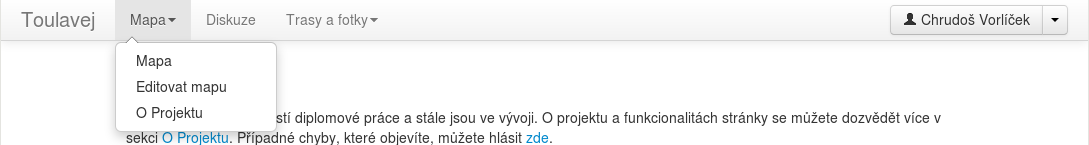
\includegraphics[width=12cm]{obrazky/toulavej/menu_puv.png}
				\caption{Původní menu}
				\label{fig:menu_puv}
			\end{center}
		\end{figure}	

		\section{Vzhled a styly}
			\paragraph{} Při tvorbě vzhledu byla snaha vytvořit jednoduché rozhraní. Z hlediska lepšího využití prostoru bylo menu navrhnuto jako lišta. Původní navigační panel\ref{fig:menu_puv} obsahoval dvě rozbalovací menu, ale po konzultaci s Ing. Landou bylo shledáno toto rozvržení nevhodným. Jednalo se např. o zařazení stránky \textit{O Projektu} pod záložku \textit{Mapa}. Předělané menu\ref{fig:menu_nove} je přehlednější.
		\begin{figure}[!h]
			\begin{center}
				
\includegraphics[width=12cm]{obrazky/toulavej/menu_nove.png}
				\caption{Nové menu}
				\label{fig:menu_nove}
			\end{center}
		\end{figure}	
			\paragraph{} Ve frameworku Bootstrap jsou vytvořeny styly pro většinu běžných prvků -- navigační lišta je jedním z nich. Díky tomu je snadné poskládat prvky do požadovaného vzhledu. Ačkoliv byl použit Bootstrap, tak pro některé prvky bylo potřeba vytvořit nové styly či upravit stávající, protože existující nevyhovovaly. Jedním z příkladů je odsazení textů. V původní verzi Bootstrapu začínal text přímo na kraji stránky, což není pro uživatele příliš příjemné. Nové styly byly většinou tvořeny pro unikátní prvky jako je např. mapové pole.
		\begin{figure}[!h]
			\begin{center}
				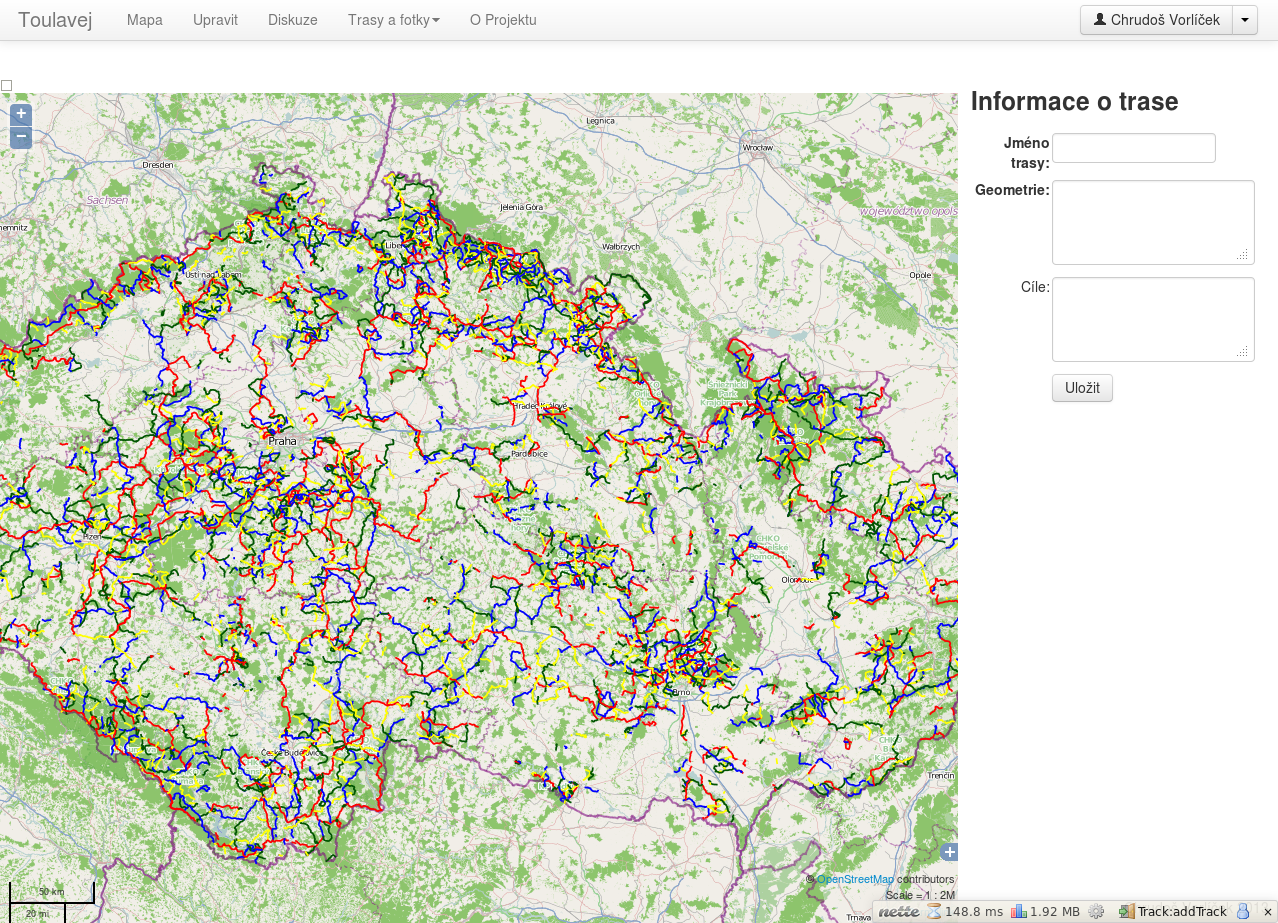
\includegraphics[width=9cm]{obrazky/toulavej/addTrack.png}
				\caption{Styl mapového pole pro přidávání tras}
				\label{fig:addTrack}
			\end{center}
		\end{figure}	
			\paragraph{} Mapových oken je v aplikaci víc a mají různá nastavení stylů. První je v samotné sekci \textit{Mapa} a hlavním rysem tohoto prvku je malé odsazení od spodního a bočních krajů. Stejný rys má i druhé okno, které se nachází v sekci \textit{Upravit}. To je ale navíc rozděleno na mapovou a textovou část. Poslední styl mapy je společný pro dvě mapová okna. Jedná se o přidání vlastní trasy a zobrazení trasy na mapě. Tento styl se vyznačuje odsazením od pravého kraje, takže zde vznikne místo pro Informace o trase -- buď vypsané v tabulce nebo vstupní formulář pro ně\ref{fig:addTrack}.
			\paragraph{} Z grafického hlediska bylo největším problémem propojení aplikace Toulavej s editorem iD. protože tato aplikace má své vlastní styly. Některé třídy stylů měly stejné názvy a  styly editoru tak přepisovaly pravidla aplikace. Tento problém byl vyřešen přepsáním pravidel, která se vzájemně rušila, tak, aby byla stejná. Ačkoliv většina aplikace byla přepsána úspěšně, v některých místech stále není úprava provedena, např. v editoru iD chybí tlačítku lokalizovat popis po najetí myši\ref{fig:error_locate}.
		\begin{figure}[!h]
			\begin{center}
				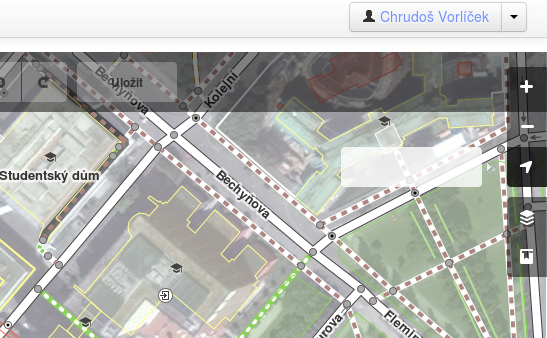
\includegraphics[width=7cm]{obrazky/toulavej/chyba_locate.png}
				\caption{Chyba stylů}
				\label{fig:error_locate}
			\end{center}
		\end{figure}	

		\section{Mapy} %Leaflet, OpenLayers v2 v3
			\paragraph{} Mapová okna mají nejen své vlastní styly, ale i své vlastní konfigurace, které bylo třeba vytvořit. Kromě připojení podkladové mapy bylo potřeba připojit i další vrstvy. První v pořadí byla připojena přes službu WFS data turistických stezek. Pro získání informací o prvku byla vytvořena funkce, která je vypíše(pokud jsou k dispozici) a zvýrazní vybranou stezku\ref{fig:infoTrack}. Informace, které mohou být zobrazeny, jsou jméno a cíle stezky, celková délka a barva trasy.
			\paragraph{} Protože načítání WFS vrstvy pro celou republiku je zdlouhavé, byla přidána WMS vrstva stezek KČT, která se při určitém přiblížení změní na dříve přidanou WFS vrstvu. Tímto se sníží čas potřebný k nahrání potřebných dat pro celou Českou republiku. Pro menší oblast je čas nahrávání vektorové vrstvy už přijatelný.
		\begin{figure}[!h]
			\begin{center}
				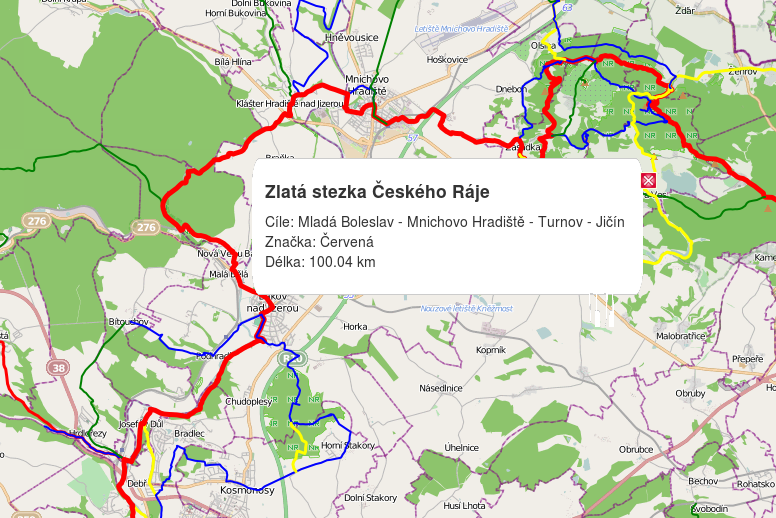
\includegraphics[width=7cm]{obrazky/toulavej/infoTrack.png}
				\caption{informace a turistické trase}
				\label{fig:infoTrack}
			\end{center}
		\end{figure}	

			\paragraph{} Abychom vůbec mohli použít WMS a WFS vrstvy z dat, která jsou uložena v databázi, musí být nastaven Geoserver, vrstvy musí být publikovány a pro WFS službu musí být na serveru přítomen soubor, který zpracovává proxy dotazy. Toto je dáno tím, že se z OpenLayers nelze připojit přímo ke Geoserveru a komunikovat s ním přímo. 
			\paragraph{} V neposlední řadě byly do mapy přidány ovládací prvky jako zoom, permanentní odkaz, měřítko a přehledka. Pokud je uživatel přihlášený, tak může pomocí funkce \textit{Editovat výřez} přejít na do editačního módu na souřadnicích, kde momentáůně leží střed mapy. Pokud má uživatel účet na Facebooku a má ho propojený s aplikací, tak může sdílet mapu s přáteli.
			\paragraph{}Pro připojení mapového HTML5 editoru iD bylo za potřebí importovat všechny knihovny a styly a nastavit autentifikační údaje pro \textit{oauth}. 

			
		\section{Uživatelské rozhraní}
			\subsection{Přihlašování uživatelů}
				\paragraph{}K ukládání registrovaných uživatelů byla v databázi vytvořena tabulka \textit{users}. Tabulka ukládá data jak uživatelů registrovaných na stránkách, tak uživatelů přihlášených přes Facebook.
				\subsubsection{Bez Facebooku}
					\paragraph{} K příhlášení bez propojení s Facebookem je potřeba se registrovat na stránce. K tomu slouží jednoduchý formulář, kde uživatel zadá požadované informace. Formulář je opatřen i pasivním filtrem proti robotům, kteří by opakovaně vytvářeli účty a zahlcovali tak databázi. Navíc by tím získali přístup k editaci dat, což je nežádoucí. Teoreticky by mohlo dojít k masovému ukládání špatných dat do OSM. 
				\subsubsection{S Facebookem}
					\paragraph{} 
			\subsection{Dostupné funkce}
				\paragraph{}

		\section{Propojení s Facebookem}
			\subsection{Použité pluginy}
				\paragraph{} Pro propojení sociální sítě Facebook s vyvíjenou aplikací byl použit plugin pro Nette\cite{nette20login} od Jakuba Marka. Tento plugin značně usnadnil tvorbu přihlašování. Dalším pluginem, který byl použit, je FbTools\cite{FbTools} od Milana Šulce. Tento plugin poskytuje funkcionality běžně dostupné na Facebooku, např. tlačítko \textit{Líbí se mi} nebo vlákno s \textit{komentáři}.
			\subsection{Práva}
				\paragraph{} Pro správné fungování funkcionalit je potřeba si vyžádat potřebná  práva. Zde se vyskytuje problém, protože toto lze nastavit pouze při prvním přihlášení uživatele. Pozdější změny jsou možné pouze tehdy, když si uživatel odebere aplikaci a poté si ji znovu přidá s novými právy. Základní právo, které je potřeba k přihlášení je \textit{email}, které povoluje získání emailu. Pro možnost publikovat na zdi, dávat \uv{lajky} a přidávat komentáře je potřeba mít právo zveřejňovat akce nazvané \textit{publish\_actions}. Toto jsou práva, o která si aplikace říká, ale nejsou jediná. Všechna práva jsou popsána v API dokumentaci\cite{FbApiPrava}.
			\subsection{Zvežejňování na zdi}
				\paragraph{} {\Huge něco o zveřejňování a sdílení}
				\paragraph{} Bylo zjištěno, že pokud se uživatel odhlásí z aplikace, ale zůstane stále přihlášen na Facebooku, tak může zveřejňovat věci na zdi. V momentě, kdy se na počítači střídá víc lidí, může dojít k situaci, kdy jeden uživatel, který vůbec nemusí mít účet na Facebooku, bude moci publikovat statusy na zdi někoho, kdo byl na počítači před ním a zapomněl se odhlásit z Facebooku. Protože toto je nežádoucí jev, byly proti němu učiněna opatření v podobě skrytí tlačítka, které sdílení vyvolávás. Tlačítko se zobrazí jen v případě, že má uživatel u svého účtu uloženo v databázi \textit{fbuid}, což je označení pro pole v tabulce \textit{user}, ve kterém je uloženo uživatelská indentifikace obdržená z Facebooku.
		
		\section{Editace dat}
				\paragraph{} Pro umožnění editace dat existovala dvě možná řešení. První řešení zahrnuje vytvoření vlastního rozhraní, druhé pak použití existujícího řešení a připojení k stávající aplikaci. U druhého řešení byla od začátku zvažována možnost použití HTML5 editoru \textit{iD}. Protože obě řešení mají své výhody a nevýhody, budou zde vypsány obě.
			\subsection{Tvorba vlastního rozhraní}
				\paragraph{} První řešení, jak už bylo řečeno, zahrnuje vytvoření jednoduchého rozhraní. Prvky by se editovaly a  ukládaly do databáze projektu a v určitých intervalech by byl prováděn import těchto dat do OpenStreetMap. Výhoda této metody spočívá v tom, že data by mohla být kontrolována, zda jsou fakticky správně, aby nedocházelo k znehodnocení dat OpenStreetMap. Také by bylo možno tuto funkci implementovat s minimálními změnami pro přidávání vlastních cest. Na druhou stranu by toto řešení znamenalo množství programování, protože by bylo potřeba zajistit nástroj pro import do OpenStreetMap, popřípadně data importovat ručně. V začátcích by to pravděpodobně nebyl problém, ovšem po překročení určitého počtu editací by se mohl stát ruční import nemožným nebo alespoň velice náročným na čas.
				\paragraph{} Protože zde nedochází k odesílání dat na jiný server, byl tento přístup zvolen pro přidávání vlastních cest.
			\subsection{Editor iD} 
				\paragraph{} Kvůli výše vyjmenovaným nevýhodám bylo rozhodnuto, že nejprve bude prozkoumána možnost připojení HTML5 editoru \textit{iD}, který byl vytvořen pro editaci dat OpenStreetMap. Po prozkoumání zdrojových kódů editoru bylo zjištěno, že aplikace může být připojena pomocí protokolu \textit{oAuth}. Aby aplikace nepoužívala osobní účet na OpenStreetMap, byl vytvořen speciální účet, pod kterým aplikace byla registrována. 
				\paragraph{}{\Large Byla snaha umožnit uživatelům s účtem na OpenStreetMap, aby mohli editovat data pod svým účtem. Zatím tato funkcionalita zprovozněna není.}
				\paragraph{} Editor iD má i určité nevýody. Například poskytuje více funkcionalit než je potřeba a komplexnost editoru činí modifikaci zdrojového kódu časově náročnou. Pro vytvářenou aplikaci je nadbytečná možnost editace budov. V momentě, kdy by nebyla povolena editace plošných prvků (polygonů), probíhalo by načítání dat z OpenStreetMap rychleji. 
		\section{Trasy a fotky}
			\paragraph{}

		\section{Testování}


%%%%%%%%%%%%%%%%%%%%%%%
%%%%% 		ZÁVĚR	  	   %%%%%
%%%%						      %%%%
%%%							  %%%
%%								     %%
%									 %
	\chapter{Zhodnocení}
		\section{Budoucí rozšíření}

		\section{Známé problémy}

		\section{MTB mapa Evropy}
			\paragraph{} V sekci Existující řešení\ref{sec:Ex_reseni} je popisována aplikace MTB mapa Evropy, která se věnuje cykloturistice a turistice. Ačkoliv aplikace zobrazují stejná data a jsou určeny pro dosti podobnou skupinu lidí, hlavní téma této práce leží v jiné oblasti než je tvorba samotné mapy. Projekt Toulavej je zaměřen hlavně na propojení se sociální sítí a s editorem iD. Stránky  nabízí možnost registrace, která poskytuje další výhody, jako je editace dat, přidávání vlastních cest a fotografií. Tyto funkce odlišují obě aplikace a nedělají z projektu Toulavej pouze další turistickou mapu. Aplikace MTB mapa Evropy byla objevena před odevzdáním této práce, a proto uvedené funkce nemohly být tvořeny jako doplňky pro stávající mapy.



%% Seznam zkratek
\newpage 
\chapter*{Seznam zkratek}
\addcontentsline{toc}{chapter}{Seznam zkratek}
	\begin{itemize}
		\item API -- Rozhraní pro programování aplikací (Application programming interface)
		\item CSS -- Kaskádové styly (Cascading Style Sheets)
		\item ČÚZK -- Český úřad zeměměřický a katastrální
		\item GNSS -- Globální navigační satelitní systém (Global navigation satellite system)
		\item GPL -- všeobecná veřejná licence (General public license)
		\item GPX -- Výměnný formát GPX (GPS eXchange format)
		\item HTML -- Hypertextový značkovací jazyk (Hypertext markup language)
		\item HTTP -- Hypertextový přenosový protokol (Hypertext transfer protocol)
		\item SLD -- Styled layer descriptor
		\item SVG -- Scalable Vector Graphics
		\item OSM -- OpenStreetMap
		\item OTM -- OpenTrackMap
		\item ÚHÚL -- Ústav pro hospodářskou úpravu lesů
		\item WFS -- Web feature service
		\item WFS-T -- Web feature service -- Transactional
		\item WMS -- Web map service
		\item WTFPL -- Veřejná licence \uv{Dělej si co do prdele chceš} (Do What The Fuck You Want To Public License)
		\item WYSIWYG -- Co vidíš je to co dostaneš (What You See Is What You Get)
	\end{itemize}



%%Užitá literatura
\newpage
\addcontentsline{toc}{chapter}{Reference}
\begin{thebibliography}{50}
	\bibitem{bootstrap}Bootstrap [online].  [cit. 2013-10-29]. Dostupné z: \url{http://getbootstrap.com}.
	\bibitem{nette20login}MAREK, Jakub: Přihlašování v Nette Frameworku [online].  [cit. 2013-10-29]. Dostupné z: \url{http://github.com/janmarek/nette20login}
	\bibitem{FbTools} ŠULC, Milan: FbTools [online].  [cit. 2013-10-29]. Dostupné z: \url{http://addons.nette.org/cs/fb-tools}.
	\bibitem{FbApiPrava} Facebook developers - Login Reference [online]. [cit. 2013-10-21]. Dostupné z: \url{https://developers.facebook.com/docs/reference/login/#permissions}.
	\bibitem{Leaflet}	Leaflet - A JavaScript Library for Mobile-Friendly Maps [online]. [cit. 2013-10-29]. Dostupné z: \url{http://leafletjs.com/}
	\bibitem{PostgreSQL} PostgreSQL: The world's most advanced open source database [online]. [cit. 2013-11-08]. Dostupné z: \url{http://www.postgresql.org/}.
	\bibitem{Waymarked} Waymarked Trails [online].  [cit. 2013-11-12]. Dostupné z: \url{http://www.waymarkedtrails.org/cs/}
	\bibitem{OTM} BARTOŇ, Radek. Custom OpenStreetMap Rendering: OpenTrackMap Experience. In: [online]. 2009. vyd. [cit. 2013-11-12]. Dostupné z: \url{http://geoinformatics.fsv.cvut.cz/gwiki/Custom_OpenStreetMap_Rendering_-_OpenTrackMap_Experience}
	\bibitem{apache}The Apache Software Foundation: Apache - HTTP Server project [online]. [cit. 2013-11-12]. Dostupné z: \url{http://httpd.apache.org/}
	\bibitem{wiki-Apache}Wikipedia:Apache HTTP Server [online]. [cit. 2013-11-12]. Dostupné z: \url{http://en.wikipedia.org/wiki/Apache_HTTP_Server}
	\bibitem{geoserver}Geoserver [online]. [cit. 2013-11-13]. Dostupné z: \url{http://geoserver.org/display/GEOS/Welcome}
	\bibitem{vorlicek}VORLÍČEK, Chrudoš: Geoportály a mapové servery v České republice, bakalářská práce. Praha: České vysoké učení technické v Praze, 2012.
	\bibitem{atlas}GeoPublishing: AtlasStyler SLD editor [online]. [cit. 2013-11-13]. Dostupné z: \url{http://en.geopublishing.org/AtlasStyler}
	\bibitem{qgis}QGIS [online]. [cit. 2013-11-13]. Dostupné z: \url{http://www.qgis.org/en/site/}
	\bibitem{postgresql} PostgreSQL [online]. [cit. 13.11.2013]. Dostupné z: \url{http://www.postgresql.org/}.
	\bibitem{mtb_map-wiki}OpenStreetMap Wiki contributors:  MTB map Europe. In OpenStreetMap Wiki [online]. [cit. 2013-12-11]. Dostupné z:\url{http://wiki.openstreetmap.org/wiki/MTB_map_Europe}.
	\bibitem{openmoko}Openmoko [online]. [cit. 12.12.2013]. Dostupné z: \url{http://geoinformatics.fsv.cvut.cz/gwiki/Custom_OpenStreetMap_Rendering_-_OpenTrackMap_Experience}
	\bibitem{otm_klic} OpenStreetMap Wiki contributors: WIKIProject Czech Republic/OTM značkový klíč. In: OpenStreetMap Wiki [online]. [cit. 2013-12-12]. Dostupné z: 	\url{http://wiki.openstreetmap.org/wiki/WikiProject_Czech_Republic/OTM_zna%C4%8Dkov%C3%BD_kl%C3%AD%C4%8D}
	\bibitem{google-wiki}Google Maps. In: Wikipedia: the free encyclopedia [online]. San Francisco (CA): Wikimedia Foundation, 2001- [cit. 2013-12-12]. Dostupné z: \url{http://en.wikipedia.org/wiki/Google_Maps}
	\bibitem{geofabrik}Geofabrik [online]. [cit. 2013-12-14] Dostupné z: \url{http://download.geofabrik.de/}.
	\bibitem{nominatim}OpenStreetMap Wiki contributors: Nominatim. In OpenStreetMap Wiki [online]. [cit. 2013-12-14]. Dostupné z: \url{http://wiki.openstreetmap.org/wiki/Nominatim}
	\bibitem{neis}NEIS, Pascal. The OpenStreetMap Contributors Map aka Who’s around me?. In: [online]. [cit. 2013-12-14]. Dostupné z: \url{http://neis-one.org/2013/01/oooc/}
	\bibitem{osm_wikipedia_cs}OpenStreetMap. In: Wikipedia: the free encyclopedia [online]. San Francisco (CA): Wikimedia Foundation, 2001- [cit. 2013-12-15]. Dostupné z: \url{http://cs.wikipedia.org/wiki/OpenStreetMap}
	\bibitem{osm_wikipedia_en}OpenStreetMap. In: Wikipedia: the free encyclopedia [online]. San Francisco (CA): Wikimedia Foundation, 2001- [cit. 2013-12-15]. Dostupné z: \url{http://en.wikipedia.org/wiki/OpenStreetMap}
	\bibitem{tesar_bp}TESAŘ, Martin. Vykreslovací systém MTB map pro OpenStreetMap. Brno, 2010. Dostupné z: \url{http://is.muni.cz/th/256369/fi_b/bpfinal.pdf}. Bakalářská práce. Masarykova univerzita. Vedoucí práce RNDr. Petr Holub, Ph.D.
	\bibitem{creative_commons}Uveďte autora-Zachovejte licenci 2.0 Generic. CREATIVE COMMONS. [online]. [cit. 2013-12-15]. Dostupné z: \url{http://creativecommons.org/licenses/by-sa/2.0/deed.cs}
	\bibitem{planet.osm}OpenStreetMap Wiki contributors: Planet.osm. In OpenStreetMap Wiki [online]. [cit. 2013-12-15]. Dostupné z: \url{http://wiki.openstreetmap.org/wiki/Planet.osm}.
	\bibitem{freemap}OpenStreetMap Wiki contributors: WIKIProject Czech Republic/freemap. In: OpenStreetMap Wiki [online]. [cit. 2013-12-15]. Dostupné z:  \url{http://wiki.openstreetmap.org/wiki/WikiProject_Czech_Republic/freemap}
	\bibitem{wiki_wtfpl} WTFPL. In: Wikipedia: the free encyclopedia [online]. San Francisco (CA): Wikimedia Foundation, 2001- [cit. 2013-12-15]. Dostupné z: \url{http://en.wikipedia.org/wiki/WTFPL}
	\bibitem{wiki_iD}OpenStreetMap Wiki contributors: iD. In: OpenStreetMap Wiki [online]. [cit. 2013-12-15]. Dostupné z:  \url{http://wiki.openstreetmap.org/wiki/ID}
	\bibitem{wiki_josm}OpenStreetMap Wiki contributors:JOSM. In: OpenStreetMap Wiki [online]. [cit. 2013-12-16]. Dostupné z:  \url{http://wiki.openstreetmap.org/wiki/JOSM}
	\bibitem{wiki_merkaator}OpenStreetMap Wiki contributors: Merkaator. In: OpenStreetMap Wiki [online]. [cit. 2013-12-16]. Dostupné z:  \url{http://wiki.openstreetmap.org/wiki/Merkaator}
	\bibitem{wiki_merkaator}OpenStreetMap Wiki contributors: Potlatch 2. In: OpenStreetMap Wiki [online]. [cit. 2013-12-16]. Dostupné z:  \url{http://wiki.openstreetmap.org/wiki/Potlatch2}
	\bibitem{wiki_comparison}OpenStreetMap Wiki contributors: Comparison of editors In: OpenStreetMap Wiki [online]. [cit. 2013-12-16]. Dostupné z:	\url{https://wiki.openstreetmap.org/wiki/Comparison_of_editors}
	\bibitem{wiki_tajfun}OpenStreetMap Wiki contributors: Typhoon Haiyan In: OpenStreetMap Wiki [online]. [cit. 2013-12-16]. Dostupné z: \url{wiki.openstreetmap.org/wiki/Typhoon_Haiyan_(2013)}
	\bibitem{wiki_hot}OpenStreetMap Wiki contributors: Humanitarian OSM Team  In: OpenStreetMap Wiki [online]. [cit. 2013-12-16]. Dostupné z: \url{http://wiki.openstreetmap.org/wiki/Humanitarian_OSM_Team}
	\bibitem{wiki_postgresql}PostgreSQL. In: Wikipedia: the free encyclopedia [online]. San Francisco (CA): Wikimedia Foundation, 2001- [cit. 2013-12-16]. Dostupné z: \url{http://en.wikipedia.org/wiki/PostgreSQL}
	\bibitem{nette_web}NETTE FOUNDATION. Nette Framework [online]. 2008. vyd. [cit. 2013-12-16]. Dostupné z: \url{http://nette.org} 
	\bibitem{wiki_ol}OpenLayers. In: Wikipedia: the free encyclopedia [online]. San Francisco (CA): Wikimedia Foundation, 2001- [cit. 2013-12-16]. Dostupné z: \url{http://en.wikipedia.org/wiki/OpenLayers}
	\bibitem{ol}OPEN SOURCE GEOSPATIAL FOUNDATION. OpenLayers: Free Maps for the Web [online]. [cit. 2013-12-17]. Dostupné z: \url{http://openlayers.org} 

\end{thebibliography}
\end{document}
